\chapter{Μεθοδολογία}
\label{Ch:methodology}
\chapterprecis{
Σε αυτό το κεφάλαιο, το θεωρητικό υπόβαθρο που αναπτύχθηκε στο \autoref{Ch:Theory} θα εφαρμοστεί για την επίλυση ενός πραγματικού προβλήματος. Το κεφάλαιο αυτό εξηγήσει το πρόβλημα που πρέπει να επιλυθεί, τον τρόπο με τον οποίο   δημιουργείται το μοντέλο αεροελαστικής ανάλυσης καθώς και τη διαδικασία που χρησιμοποιείται για τη βελτιστοποίηση του.}

\section{Εισαγωγή στο Πρόβλημα}
\label{problem-introduction}

Το πρόβλημα που έχει επιλεγεί ως παράδειγμα εφαρμογής της θεωρίας που αναπτύχθηκε στο προηγούμενο κεφάλαιο είναι η μελέτη των χαρακτηριστικών πτερυγισμού της κύριας πτέρυγας του ανεμοπλάνου \textlatin{ASW 28} και η  βελτιστοποίηση του σχεδιασμού, του σύνθετου υλικού του για να προσαρμοστούν τα χαρακτηριστικά του πτερυγισμού σε συγκεκριμένες απαιτήσεις. Η επιλογή αυτού του συγκεκριμένου αεροσκάφους έγινε λόγω του μεγάλου εκπετάσματος σε σχέση με το μήκος της χορδής του \textlatin{aspect ratio}, γεγονός που το καθιστά πολύ ευλύγιστο. Επιπλέον, ο κύριος στόχος ενός ανεμοπλάνου είναι να επιτύχει τo βέλτιστo λόγο καθόδου \textlatin{glide ratio}, επομένως η μείωση του βάρους είναι υψίστης σημασίας για αυτά τα οχήματα κάτι που τα καθιστά ιδανικά για αυτήν την εφαρμογή καθώς συνδυάζουν τη μεγάλη πιθανότητα εμφάνισης πτερυγισμού με την ανάγκη για ελαχιστοποίηση βάρους.

\textlatin{``The ASW 28 is Schleicher's high-performance glider for the
FAI-Standard Class with 15m span.'' \cite{asw28}}. Τα τεχνικά χαρακτηριστικά αυτού του αεροσκάφους συνοψίζονται στο \autoref{fig:TechnicalDataofASW28glider} :


\begin{figure}[H]
\centering
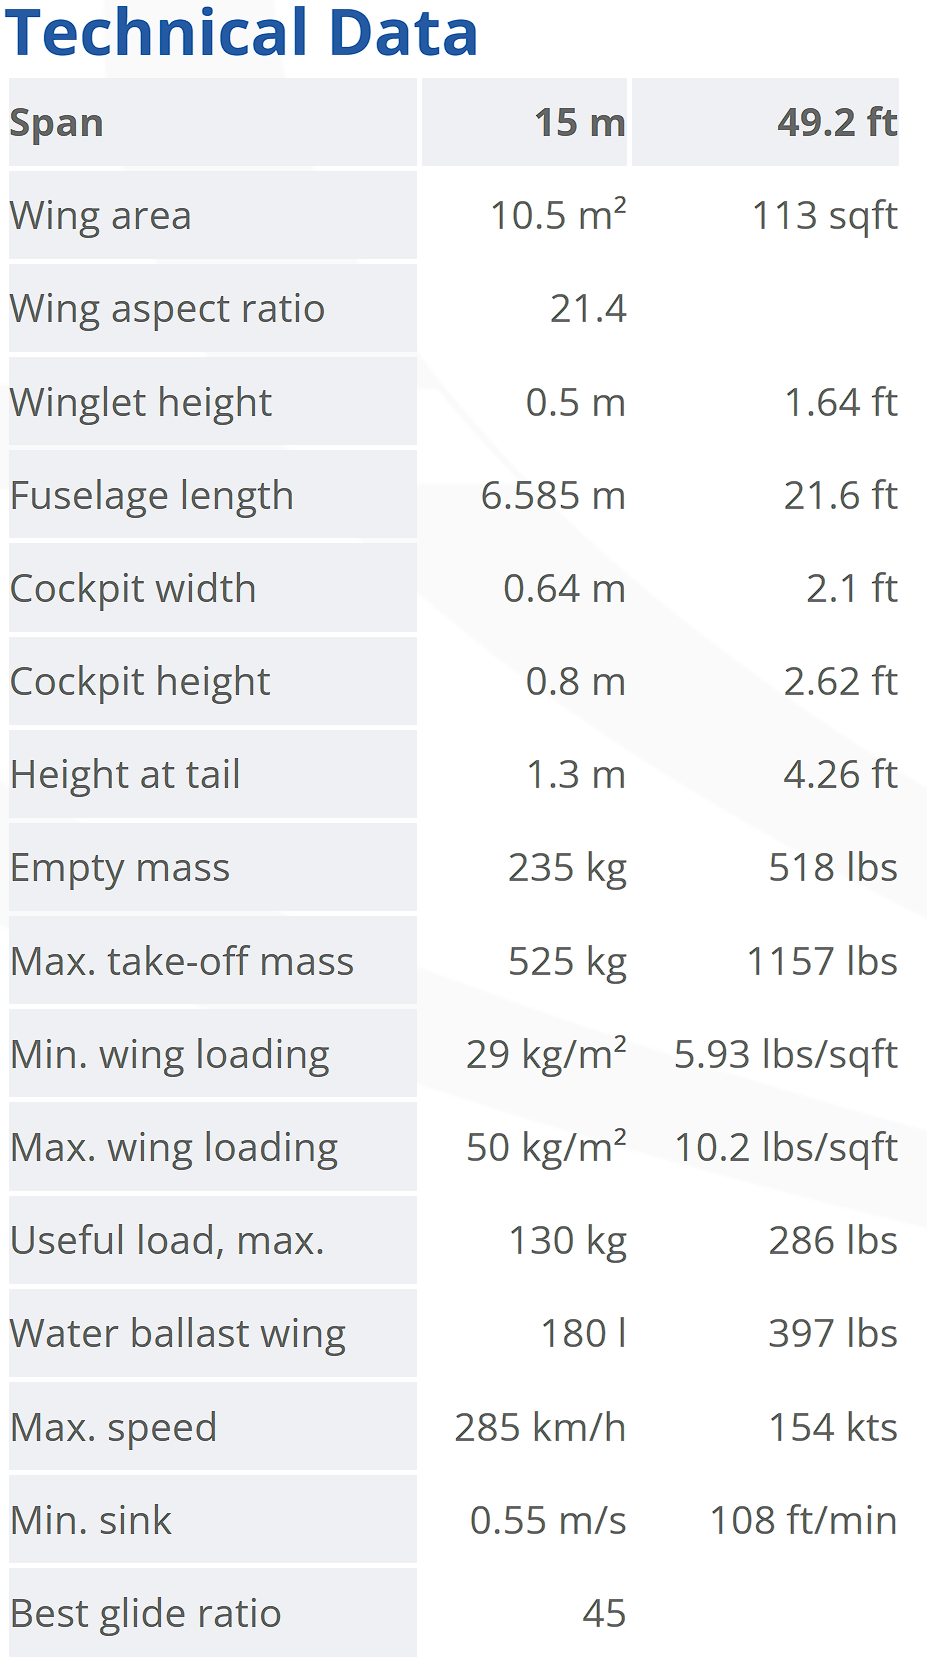
\includegraphics[width=2.92073in]{ASW28_characteristics.png}
\caption{Τεχνικά δεδομένα του ανεμοπλάνου \textlatin{ASW 28 \cite{asw28}}}
\label{fig:TechnicalDataofASW28glider}
\end{figure}

\begin{figure}[H]
\centering
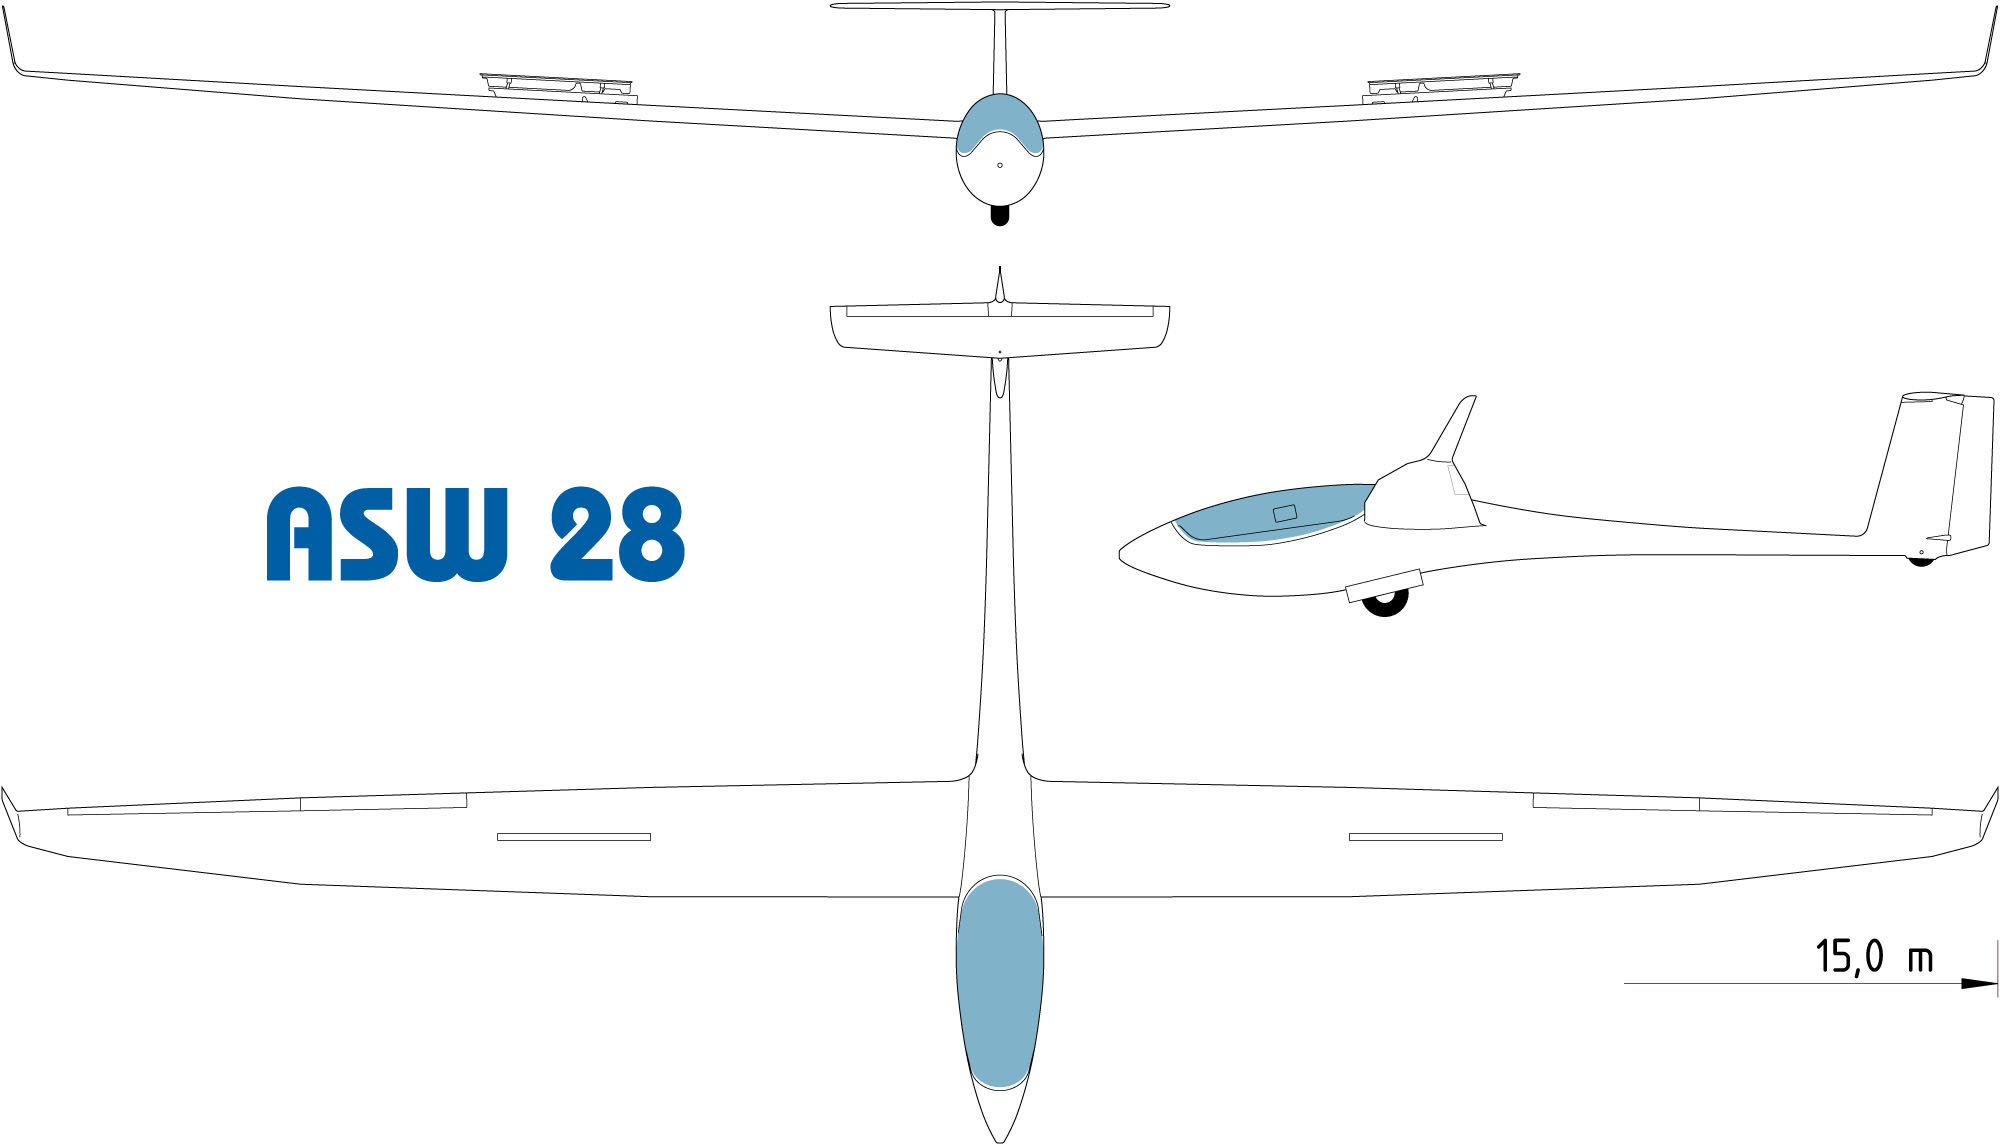
\includegraphics[width=5.5026in,height=3.34935in]{ASW 28 3side view.png}
\caption{Εμπρόσθια, πλάγια και άνω όψη του ανεμοπλάνου  \textlatin{ASW 28 \cite{asw28}}}
\end{figure}

Η ανάλυση της κύριας πτέρυγας του \textlatin{ASW 28} θα περιλαμβάνει τα εξής βήματα:

\begin{enumerate}
  \def\labelenumi{\arabic{enumi}.}
  \item
    Δημιουργία μοντέλου στο \textlatin{HyperMesh} της \textlatin{Altair} για ανάλυση ιδιομορφών και πτερυγισμού.
  \item
    Δημιουργία κώδικα σε \textlatin{Python} για το αυτόματο διάβασμα των αποτελεσμάτων πτερυγισμού από τον επιλυτή \textlatin{Optistruct}.
  \item
    Ορισμός του προβλήματος βελτιστοποίησης χρησιμοποιώντας διάφορες τεχνικές βελτιστοποίησης και υλοποίηση αυτών με \textlatin{Python}.
  \end{enumerate}
  
  

  \section{Μοντέλο Κύριας Πτέρυγας \textlatin{ASW 28}}
  \label{asw-28-main-composite-wing-model}
  
  \subsection{Γεωμετρία Πτέρυγας \&\ Διακριτοποίηση Γεωμετρίας}\label{wing-geometry-discretization}
  
  Η εξωτερική γεωμετρία της πτέρυγας εισήχθη στο \textlatin{HyperMesh} από ένα αρχείο \textlatin{CAD}. Η γεωμετρία καθαρίστηκε ώστε να περιλαμβάνει μόνο την κύρια πτέρυγα του αεροσκάφους και λόγω ορισμένων ανακριβειών και των μη μετρικών μονάδων μήκους που χρησιμοποιήθηκαν στο \textlatin{CAD}, χρειάστηκε να γίνει μετασχηματισμός κλίμακας. Η εξωτερική γεωμετρία παρουσιάζεται στο \autoref{fig:externalGemometryASW28}
  

\begin{figure}[H]
    \centering
    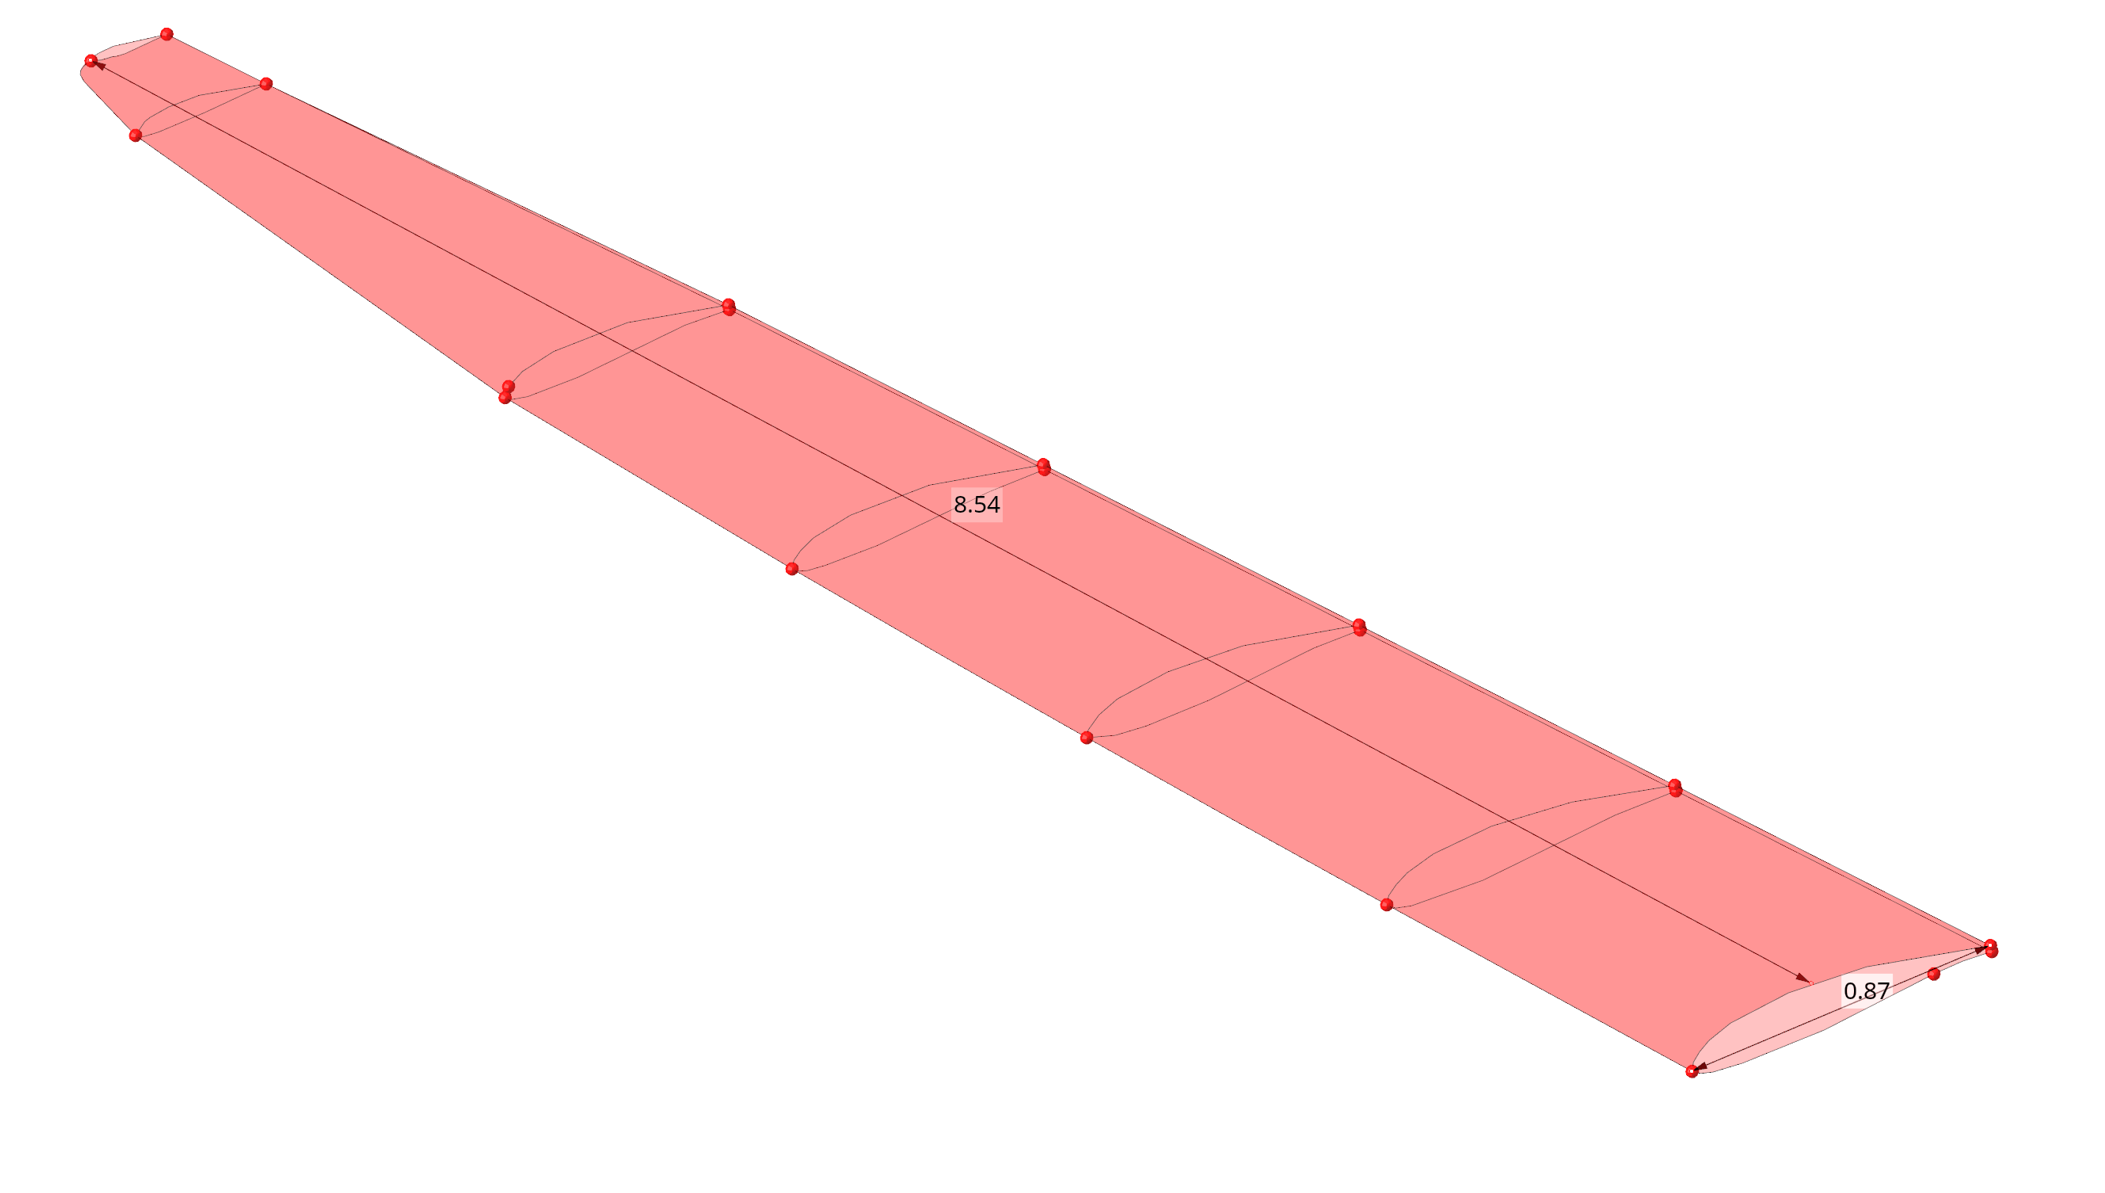
\includegraphics[width=\textwidth]{ASW 28 External Geometry.png}
    \caption{Εξωτερική Γεωμετρία της πτέρυγας του \textlatin{ASW 28} \textlatin{(length in meters)}}
    \label{fig:externalGemometryASW28}
\end{figure}

Μετά τη δημιουργία της εξωτερικής γεωμετρίας, η εσωτερική δομή της πτέρυγας έπρεπε να δημιουργηθεί από την αρχή. Εφόσον τα λεπτομερή σχέδια της εσωτερικής δομής δεν είναι διαθέσιμα, η γεωμετρία της εσωτερικής δομής υποτέθηκε με βάση κάποιες φωτογραφίες της αποσυναρμολογημένης πτέρυγας. Τα κύρια χαρακτηριστικά της εσωτερικής γεωμετρίας των περισσότερων σύγχρονων πτερύγων είναι τα \textlatin{spars} και τα \textlatin{ribs}. Τα \textlatin{spars} είναι το κύριο δομικό στοιχείο της πτέρυγας που εκτείνονται κατά μήκος της πτέρυγας και είναι υπεύθυνα για τη μεταφορά των αεροδυναμικών φορτίων στο αεροπλάνο. Τα \textlatin{ribs} είναι δομικά μέλη της πτέρυγας που εκτείνονται κατά μήκος της χορδής και ο σκοπός τους είναι να υποστηρίζουν το εξωτερικό περίβλημα της πτέρυγας έτσι ώστε να διατηρεί το σωστό προφίλ αεροτομής.

Οι σύγχρονες πτέρυγες ανεμόπτερων συνήθως έχουν μόνο ένα \textlatin{spar} και αρκετά \textlatin{ribs}. Για αυτήν την εφαρμογή χρησιμοποιούνται ένα \textlatin{spar} ορθογώνιας διατομής που στενεύει προς την άκρη της πτέρυγας και 6 \textlatin{ribs} που απεικονίζονται στο \autoref{fig:ASW 28 Wing Internal geometry}.

\begin{figure}[H]
    \centering
    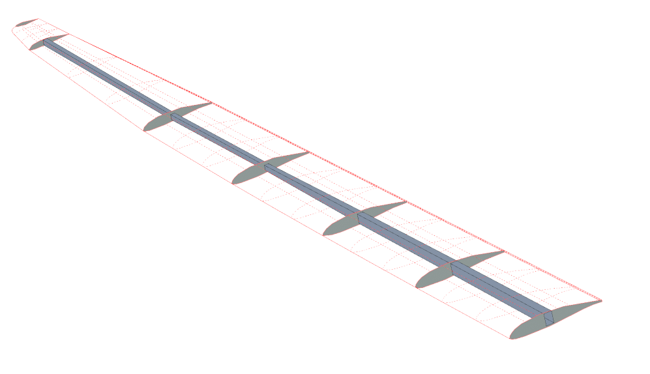
\includegraphics[width=\textwidth]{ASW 28 Internal Geometry.png}
    \caption{Εσωτερική Γεωμετρία της πτέρυγας του \textlatin{ASW 28}}
    \label{fig:ASW 28 Wing Internal geometry}
\end{figure}


Η διακριτοποίηση της γεωμετρίας επιτεύχθηκε χρησιμοποιώντας επιφανειακά στοιχεία που τοποθετήθηκαν σε ένα πλέγμα το οποίο δημιουργήθηκε με τη βοήθεια του εργαλείου \textlatin{``Panel Mesh''} του \textlatin{HyperMesh} για το περίβλημα της πτέρυγας, καθώς αυτή η λειτουργία είναι ιδιαίτερα κατάλληλη για αυτόν τον τύπο γεωμετρίας που μοιάζει με πάνελ, και του εργαλείου \textlatin{``General 2D Mesh''} για τη εσωτερική γεωμετρία. Το μέσο μέγεθος των στοιχείων έχει μήκος πλευράς \(0.02\ [m]\).

Η διακριτοποίηση δεν χρειάζεται να είναι πολύ ακριβής, καθώς για την ανάλυση του πτερυγισμού χρειάζεται μόνο τόση λεπτομέρεια ώστε να περιγραφούν οι πρώτες ιδιομορφές ενώ δεν μας ενδιαφέρουν οι ακριβείς τάσεις σε συγκεκριμένα σημεία μέσα στη δομή. Η διακριτοποίση της γεωμετρίας σε πεπερασμένα στοιχεία φαίνεται στα Σχήματα \ref{fig:ASW 28 Wing Internal mesh} και \ref{fig:ASW 28 Wing skin mesh}.


\begin{figure}[H]
\centering
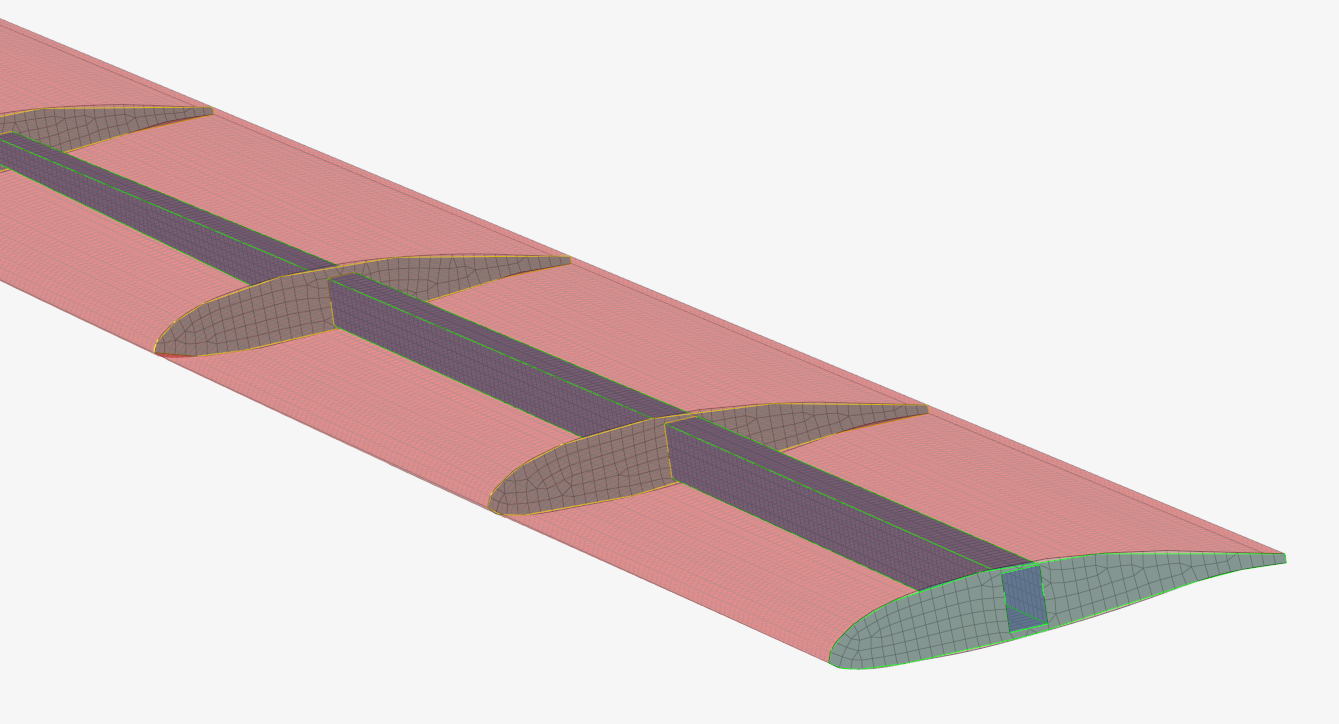
\includegraphics[width = \textwidth]{ASW 28 Wing Mesh.png}
\caption{Διακριτοποίηση Εσωτερικής Γεωμετρίας της πτέρυγας του \textlatin{ASW 28}}
\label{fig:ASW 28 Wing Internal mesh}

\end{figure}

\begin{figure}[H]
\centering
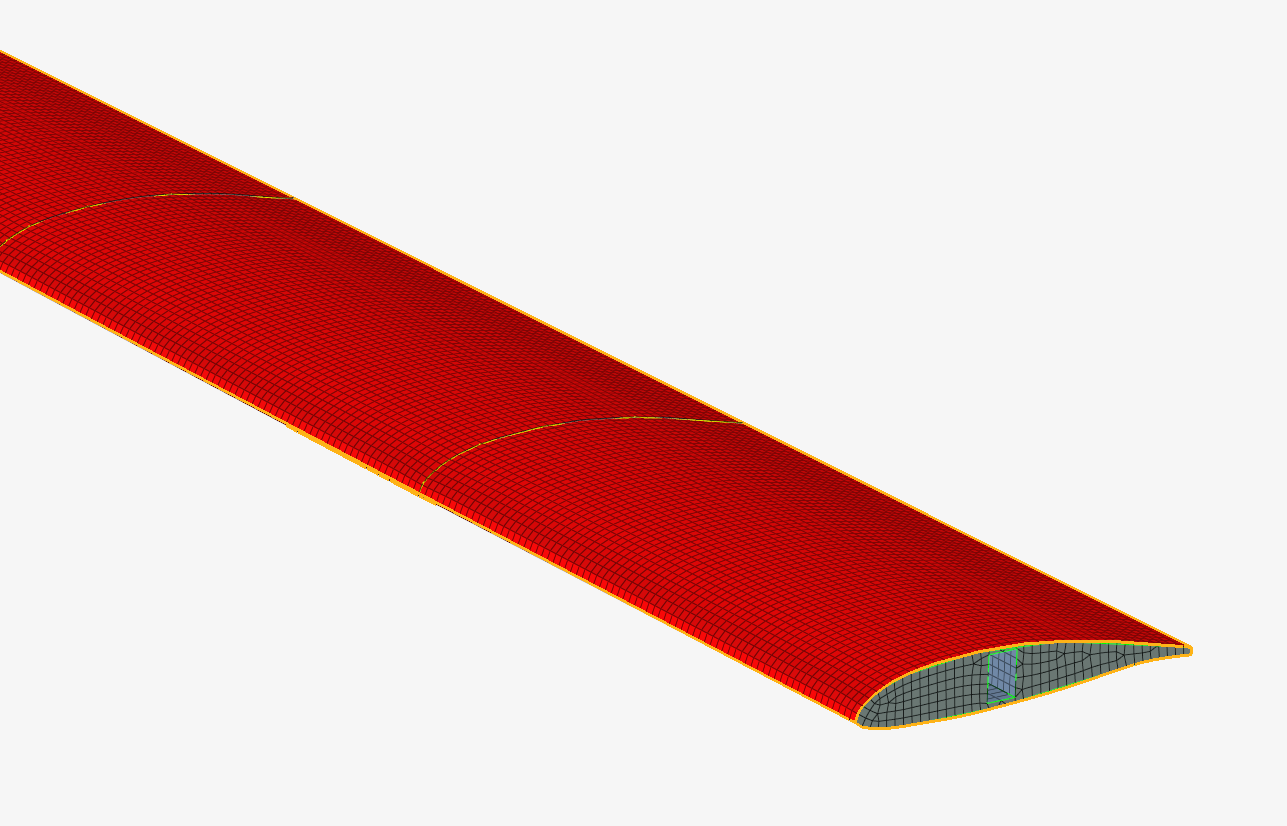
\includegraphics[width = \textwidth]{ASW 28 Wing Skin Mesh.png}
\caption{Διακριτοποίηση Εξωτερικής Γεωμετρίας της πτέρυγας του \textlatin{ASW 28}}
\label{fig:ASW 28 Wing skin mesh}
\end{figure}

\subsection{Ορισμός Ιδιοτήτων Υλικών}
\label{material-properties-definition.}

Οι ιδιότητες των υλικών που χρησιμοποιήθηκαν στην πτέρυγα είναι κάπως αυθαίρετες, καθώς αυτές οι πληροφορίες δεν είναι διαθέσιμες δημοσίως. Αυτό δε θα δημιουργήσει προβλήματα στο στόχο της παρούσας διατριβής, καθώς κατά τη διάρκεια της βελτιστοποίησης, οι ιδιότητες των υλικών είναι πιθανό να αλλάξουν ούτως ή άλλως ενώ κύριος σκοπός της διατριβής είναι η ανάπτυξη της μεθοδολογίας και όχι η συγκεκριμένη εφαρμογή.

Ένα κοινό σύνθετο υλικό για το εξωτερικό των  ανεμόπτερων υψηλών επιδόσεων είναι το \textlatin{fiberglass} ή τα ανθρακονήματα, καθώς αυτά τα υλικά προσφέρουν υψηλή αντοχή, χαμηλό βάρος και μια λεία αεροδυναμική επιφάνεια. Για αυτήν την εφαρμογή επιλέχθηκε ένα σύνθετο υλικό από ανθρακόνημα - \textlatin{Epoxy}. Για τον επιλυτή \textlatin{Optistruct}, αυτός ο τύπος σύνθετου υλικού μπορεί να οριστεί χρησιμοποιώντας την κάρτα υλικού \textlatin{MAT8} με τις παρακάτω ιδιότητες \cite{matweb}:


\begin{itemize}
\item
  \(E_{1} = 125\ GPa\)
\item
  \(E_{2} = 8.41GPa\)
\item
  \(\nu_{12} = 0.35\)
\item
  \(G_{12} = 4.23\ GPa\)
\item
  \(\rho = 1517\ kg\text{/}m^{3}\)
\end{itemize}

Αυτό το υλικό είναι ένα \textlatin{laminated composite} και αν και οι ιδιότητες του υλικού έχουν καθοριστεί επαρκώς, η δομή του \textlatin{layup} δεν είναι ακόμη ορισμένη. Για να οριστεί το \textlatin{layup}, απαιτείται η κάρτα ιδιότητας \textlatin{PCOMP}. Αυτή η κάρτα είναι ουσιαστικά μια λίστα που περιέχει τις ιδιότητες κάθε στρώσης του \textlatin{laminate}. Οι ιδιότητες αυτές είναι:

\begin{enumerate}
  \def\labelenumi{\arabic{enumi}.}
  \item
    Το υλικό της στρώσης του \textlatin{laminate} ορίζεται ως κάρτα σύνθετου υλικού, στην προκειμένη περίπτωση μια κάρτα \textlatin{MAT8}.
  \item
    Το πάχος κάθε στρώσης του \textlatin{laminate} ορίζεται ως πραγματικός αριθμός.
  \item
    Η γωνία σε μοίρες του κύριου άξονα (άξονας 1) της στρώσης του \textlatin{laminate}.
  \end{enumerate}
  
  Για αυτήν την εφαρμογή θα δημιουργηθεί ένα σύνθετο υλικό με έξι στρώσεις \textlatin{laminate} χρησιμοποιώντας \textlatin{carbon-fiber epoxy} ορθοτροπικό υλικό με γωνίες που εναλλάσσονται μεταξύ $+45$ και $-45$ μοίρες και πάχος \(0.5\ mm\) για κάθε στρώση.
  
  Για την εσωτερική δομή της πτέρυγας χρησιμοποιείται αλουμίνιο. Πιο συγκεκριμένα, χρησιμοποιείται το αλουμίνιο 6061, το οποίο έχει τις παρακάτω ιδιότητες:
  

\begin{itemize}
\item
  \(E = 69\ GPa\)
\item
  \(\nu = 0.33\)
\item
  \(\rho = 2700\ kg\text{/}m^{3}\)
\end{itemize}

Αυτό είναι ένα ισοτροπικό υλικό και ορίζεται στο \textlatin{Optistruct} με μια κάρτα MAT1, η οποία ουσιαστικά παραθέτει αυτές τις παραμέτρους του υλικού με συγκεκριμένο τρόπο.

Ομοίως, μόνο ο ορισμός του υλικού δεν είναι επαρκής. Καθώς δουλεύουμε με επιφανειακά στοιχεία, πρέπει να οριστεί και το πάχος τους. Στο \textlatin{Optistruct} αυτή η ιδιότητα ορίζεται χρησιμοποιώντας μια κάρτα ιδιότητας \textlatin{PSHELL}, η οποία χρειάζεται  να περιέχει μόνο μια αναφορά στο υλικό και σε μια τιμή πάχους. Στην προκειμένη περίπτωση, το πάχος είναι ομοιόμορφο παντού και ισούται με \(t = 2mm\).


\subsection{Συνοριακές Συνθήκες} \label{boundary-conditions}

Οι συνοριακές συνθήκες που ορίζονται για αυτό το πρόβλημα είναι παρόμοιες με αυτές μιας πακτωμένης -- ελεύθερης δοκού. Οι κόμβοι στη ρίζα της πτέρυγας πακτώνονται σε κάθε βαθμό ελευθερίας με  \textlatin{SPC's (Single Point Constraints)}. Αυτές οι συνοριακές συνθήκες υποθέτουν ότι η ρίζα της πτέρυγας είναι τελείως σταθερή, κάτι που λειτουργεί καλά για μια αποσπασμένη πτέρυγα που βρίσκεται σε πειραματική διάταξη, αλλά είναι μόνο μια προσέγγιση της πραγματικής κατάστασης κατά την πτήση, όπου η πτέρυγα είναι στερεωμένη στο αεροπλάνο, το οποίο δεν είναι στατικό κατά την πτήση. Οι συνοριακές συνθήκες φαίνονται στο \autoref{fig:ASW 28 Wing Boundary conditions}


\begin{figure}[H]
\centering
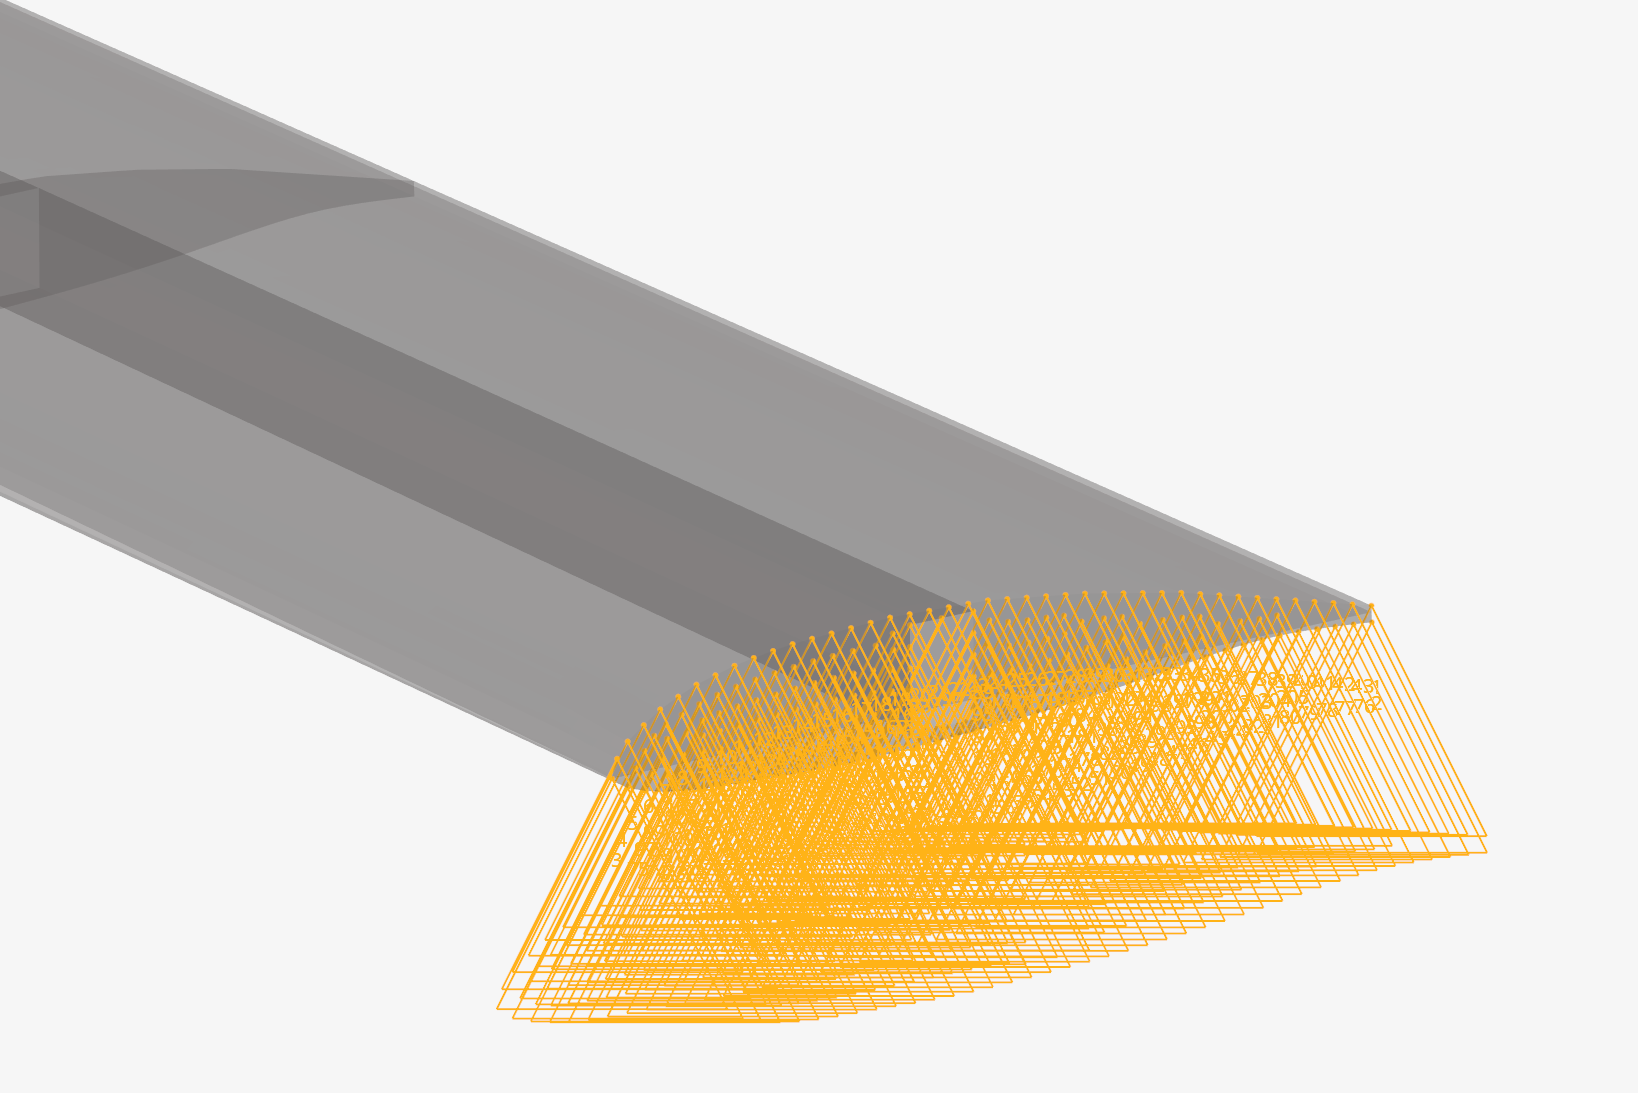
\includegraphics[width = \textwidth]{ASW 28 SPC.png}
\caption{Συνοριακές συνθήκες της πτέρυγας του \textlatin{ASW 28} }
\label{fig:ASW 28 Wing Boundary conditions}

\end{figure}

\subsection{Αεροδυναμικό Πλέγμα}
\label{aerodynamic-grid}

Για να δημιουργηθεί το πλέγμα \textlatin{vortex-lattice}, η αεροδυναμική επιφάνεια της πτέρυγας πρέπει να διακριτοποιηθεί. Ο τρόπος με τον οποίο μοντελοποιείται αυτό στο \textlatin{Optistruct} είναι μέσω της κάρτας \textlatin{CAERO1}, η οποία ορίζει ένα ((αεροδυναμικό μακρο-στοιχείο)) με απλή δισδιάστατη γεωμετρία τετραπλεύρου που χωρίζεται σε έναν προεπιλεγμένο αριθμό απο \textlatin{boxes} στις κατευθύνσεις του άξονα κατα μήκος της χορδής και του διαμήκη άξονα της πτέρυγας. Για να οριστεί η κάρτα \textlatin{CAERO1}, πρέπει πρώτα να οριστούν τα τέσσερα σημεία γωνίας με συγκεκριμένη σειρά:


\begin{itemize}
  \item
    Το πρώτο σημείο βρίσκεται στην ακμή προσβολής και στη ρίζα της πτέρυγας.
  \item
    Το δεύτερο σημείο έχει την ίδια συντεταγμένη \(y\) με το πρώτο, αλλά βρίσκεται στην ακμή φυγής της πτέρυγας.
  \item
    Το τρίτο σημείο βρίσκεται στην άκρη της πτέρυγας και στην ακμή φυγής.
  \item
    Το τέταρτο σημείο έχει την ίδια συντεταγμένη \(y\) με το τρίτο, αλλά βρίσκεται στην ακμή προσβολής της άκρης της πτέρυγας.
\end{itemize}

Τα σημεία αυτά φαίνονται στο \autoref{fig:Coordinate System of CAERO1 Aerodynamic panel} 
  

\begin{figure}[H]
    \centering
    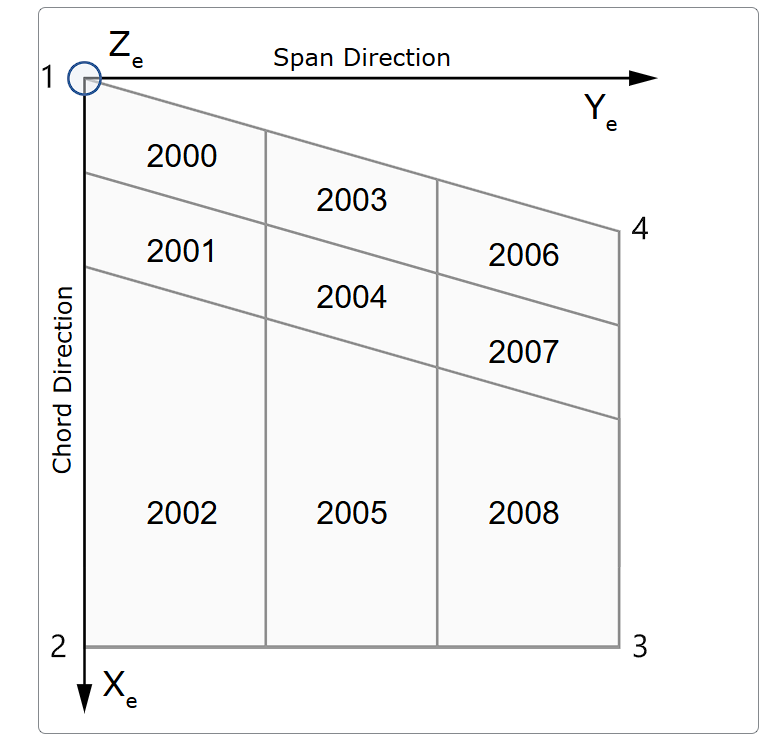
\includegraphics[width=0.6\textwidth]{CAERO1 Coordinate system.png}
    \caption{Σύστημα συντεταγμένων ενός \textlatin{CAERO1 Aerodynamic panel \cite{altair_flutter_tips}}}
    \label{fig:Coordinate System of CAERO1 Aerodynamic panel}

\end{figure}


Αυτό επιτρέπει τη μοντελοποίηση μόνο απλών γεωμετριών τραπεζοειδούς σχήματος. Επειδή η προβολή της πτέρυγας του ανεμόπτερου \textlatin{ASW28} στο επίπεδο $XY$ δεν ταιριάζει καλά μέσα σε ένα μόνο τραπεζοειδές σχήμα, χρησιμοποιήθηκαν δύο από αυτά τα μακρο-στοιχεία για να αποτυπωθεί η μεταβαλλόμενη οπισθόκληση αυτής της πτέρυγας. Αυτά τα πάνελ φαίνονται στο \autoref{fig:CAERO1 macro elements of the ASW 28 Wing Model}.


\begin{figure}[H]
\centering
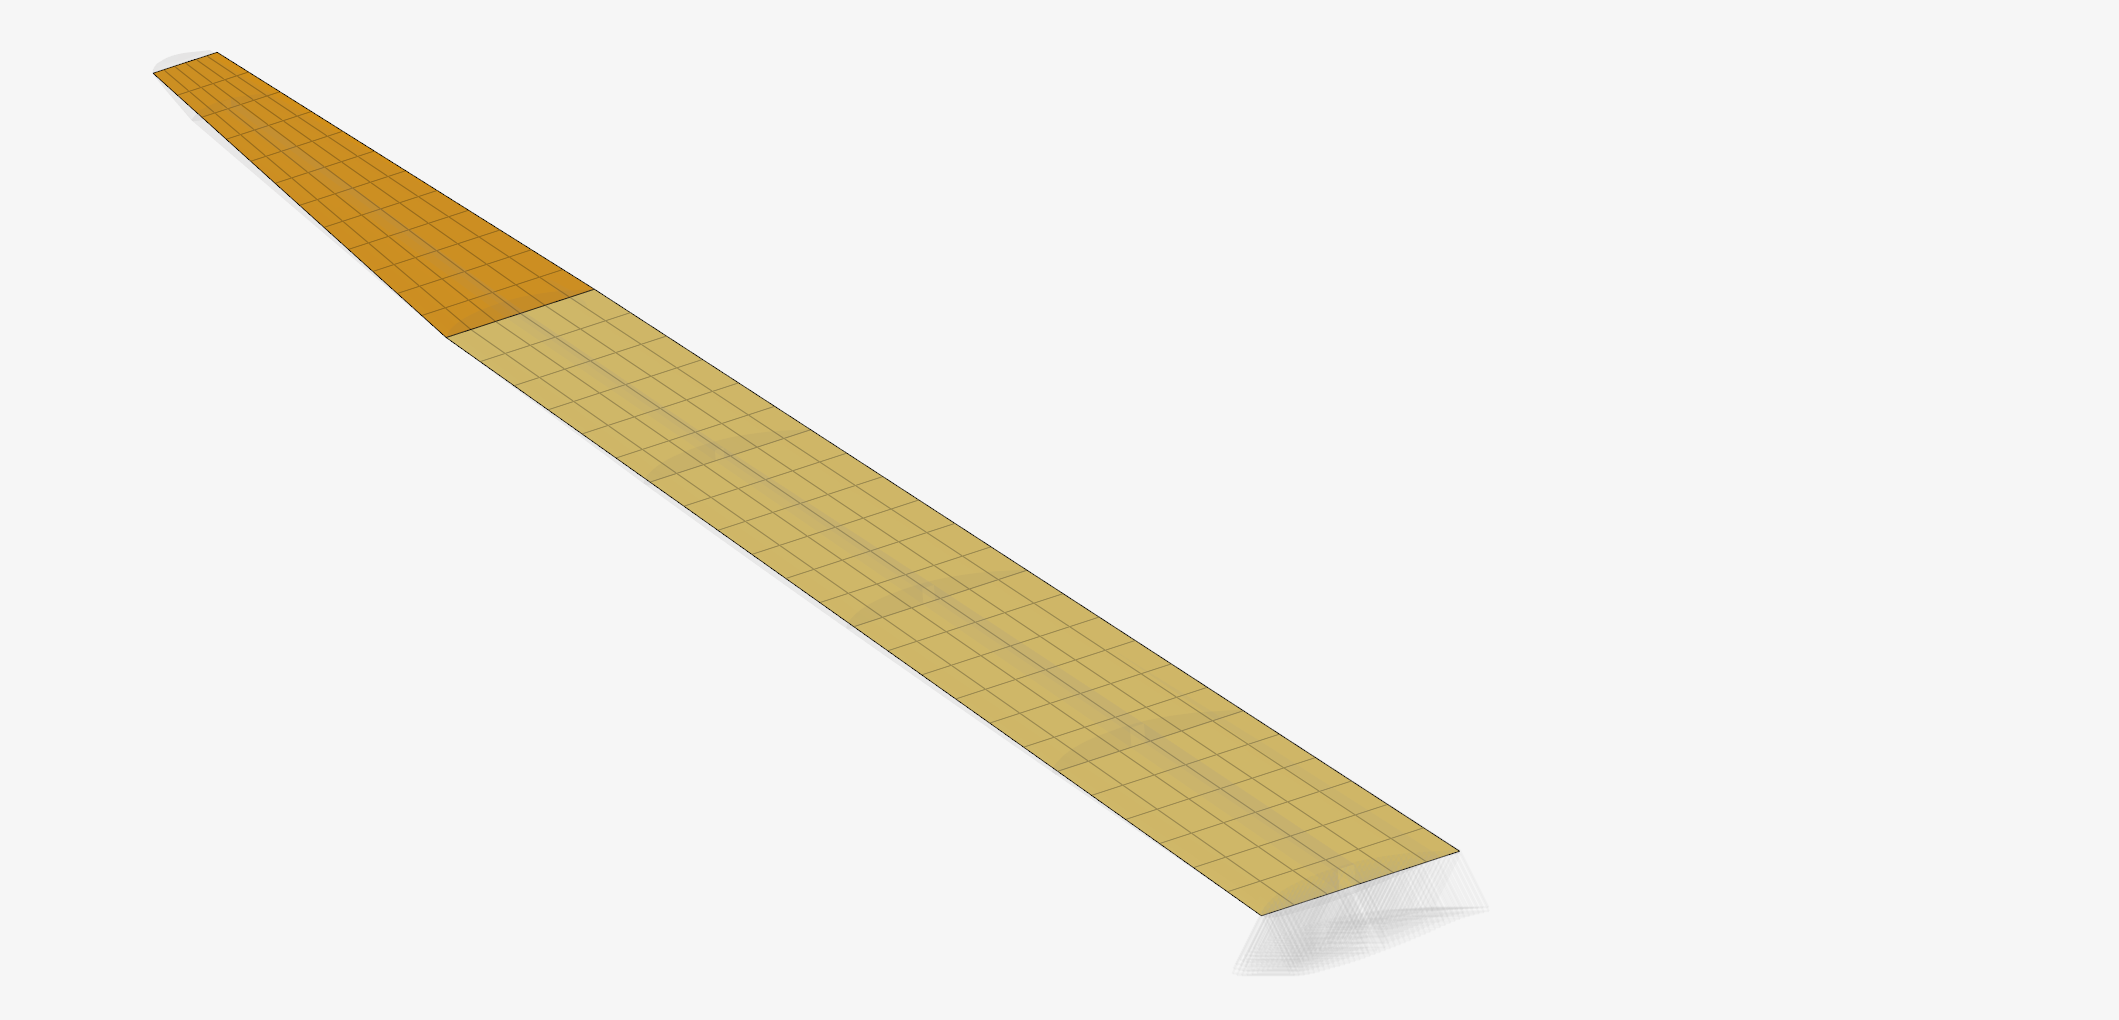
\includegraphics[width=4.65278in,height=3.01736in]{ASW 28 Aerodynamic grid.png}
\caption{ Τα \textlatin{CAERO1 macro elements} της πτέρυγας του \textlatin{ASW 28}}
\label{fig:CAERO1 macro elements of the ASW 28 Wing Model}

\end{figure}

Το επόμενο βήμα για τον ορισμό των στοιχείων \textlatin{CAERO1} είναι ο ορισμός της διακριτοποίησης σε αεροδυναμικά \textlatin{boxes} μέσω δύο ακέραιων τιμών \(NSAPN\) και \(NCHORD\), οι οποίες ορίζουν τον αριθμό των \textlatin{boxes} κατά μήκος της πτέρυγας και της χορδής αντίστοιχα.

Για το εσωτερικό μακρο-στοιχείο \textlatin{CAERO1}:

\[NSPAN = 24,\ \ NCHORD = 6\]

Για το εξωτερικό μακρο-στοιχείο CAERO1:

\[NSPAN = 12,\ \ NCHORD = 6\]

Αυτή η διακριτοποίηση επιλέγεται έτσι ώστε ο λόγος διαστάσεων των \textlatin{boxes} να είναι μικρότερος από τρία περίπου και το μήκος της χορδής κάθε κουτιού να είναι μικρότερο από \(\Delta x < 0.08V_{\max}\ \text{/}f_{\max} \approx 0.65m\). Αυτές οι δύο συστάσεις για τη διακριτοποίηση των αεροδυναμικών πάνελ γίνονται στο εγχειρίδιο του \textlatin{Nastran} \cite{msc2021}.


\subsection{Η διασυνδετική καμπύλη \textlatin{Spline}} \label{the-spline}

Στην ανάλυση πτερυγισμού, η κάρτα \textlatin{SPLINE} χρησιμοποιείται για να συνδέσει τον κατασκευαστικό και τον αεροδυναμικό τομέα. Για αυτή την εφαρμογή χρησιμοποιείται η κάρτα \textlatin{SPLINE1}, η οποία ορίζει ένα επιφανειακό \textlatin{spline} (μονοδιάστατα \textlatin{spline} είναι επίσης διαθέσιμα, αλλά δεν εφαρμόζονται σε αυτή την περίπτωση). Για να οριστεί η κάρτα \textlatin{SPLINE1} απαιτούνται οι εξής καταχωρίσεις:

\begin{itemize}
\item
  Το \textlatin{Id} του \textlatin{CAERO} που ορίστηκε στο προηγούμενο βήμα.
\item
  Τα \textlatin{Id} των πρώτων και τελευταίων αεροδυναμικών \textlatin{boxes} που πρέπει να συμπεριληφθούν (όλα τα αεροδυναμικά πάνελ επιλέγονται για αυτή την ανάλυση).
\item
  Ένα σύνολο κόμβων από το δομικό πλέγμα.
\end{itemize}

Η επιλογή των κατασκευαστικών κόμβων είναι σημαντική. Συνήθως, δεν επιλέγονται όλοι οι κόμβοι του μοντέλου. Επιλέγεται μόνο ένα υποσύνολο των κόμβων στην κάτω ή την άνω επιφάνεια της πτέρυγας. Αυτοί οι κόμβοι πρέπει να βρίσκονται στην περιοχή που καλύπτεται από τα  \textlatin{CAERO} μακρο-στοιχεία και τα αεροδυναμικά \textlatin{boxes} που επιλέχθηκαν. Ιδανικά, κάθε αεροδυναμικό σημείο του πλέγματος έχει έναν αντίστοιχο κατασκευαστικό κόμβο ακριβώς από πάνω ή από κάτω του, αν και αυτό δεν είναι εφικτό στις περισσότερες περιπτώσεις.


\begin{figure}[H]
\centering
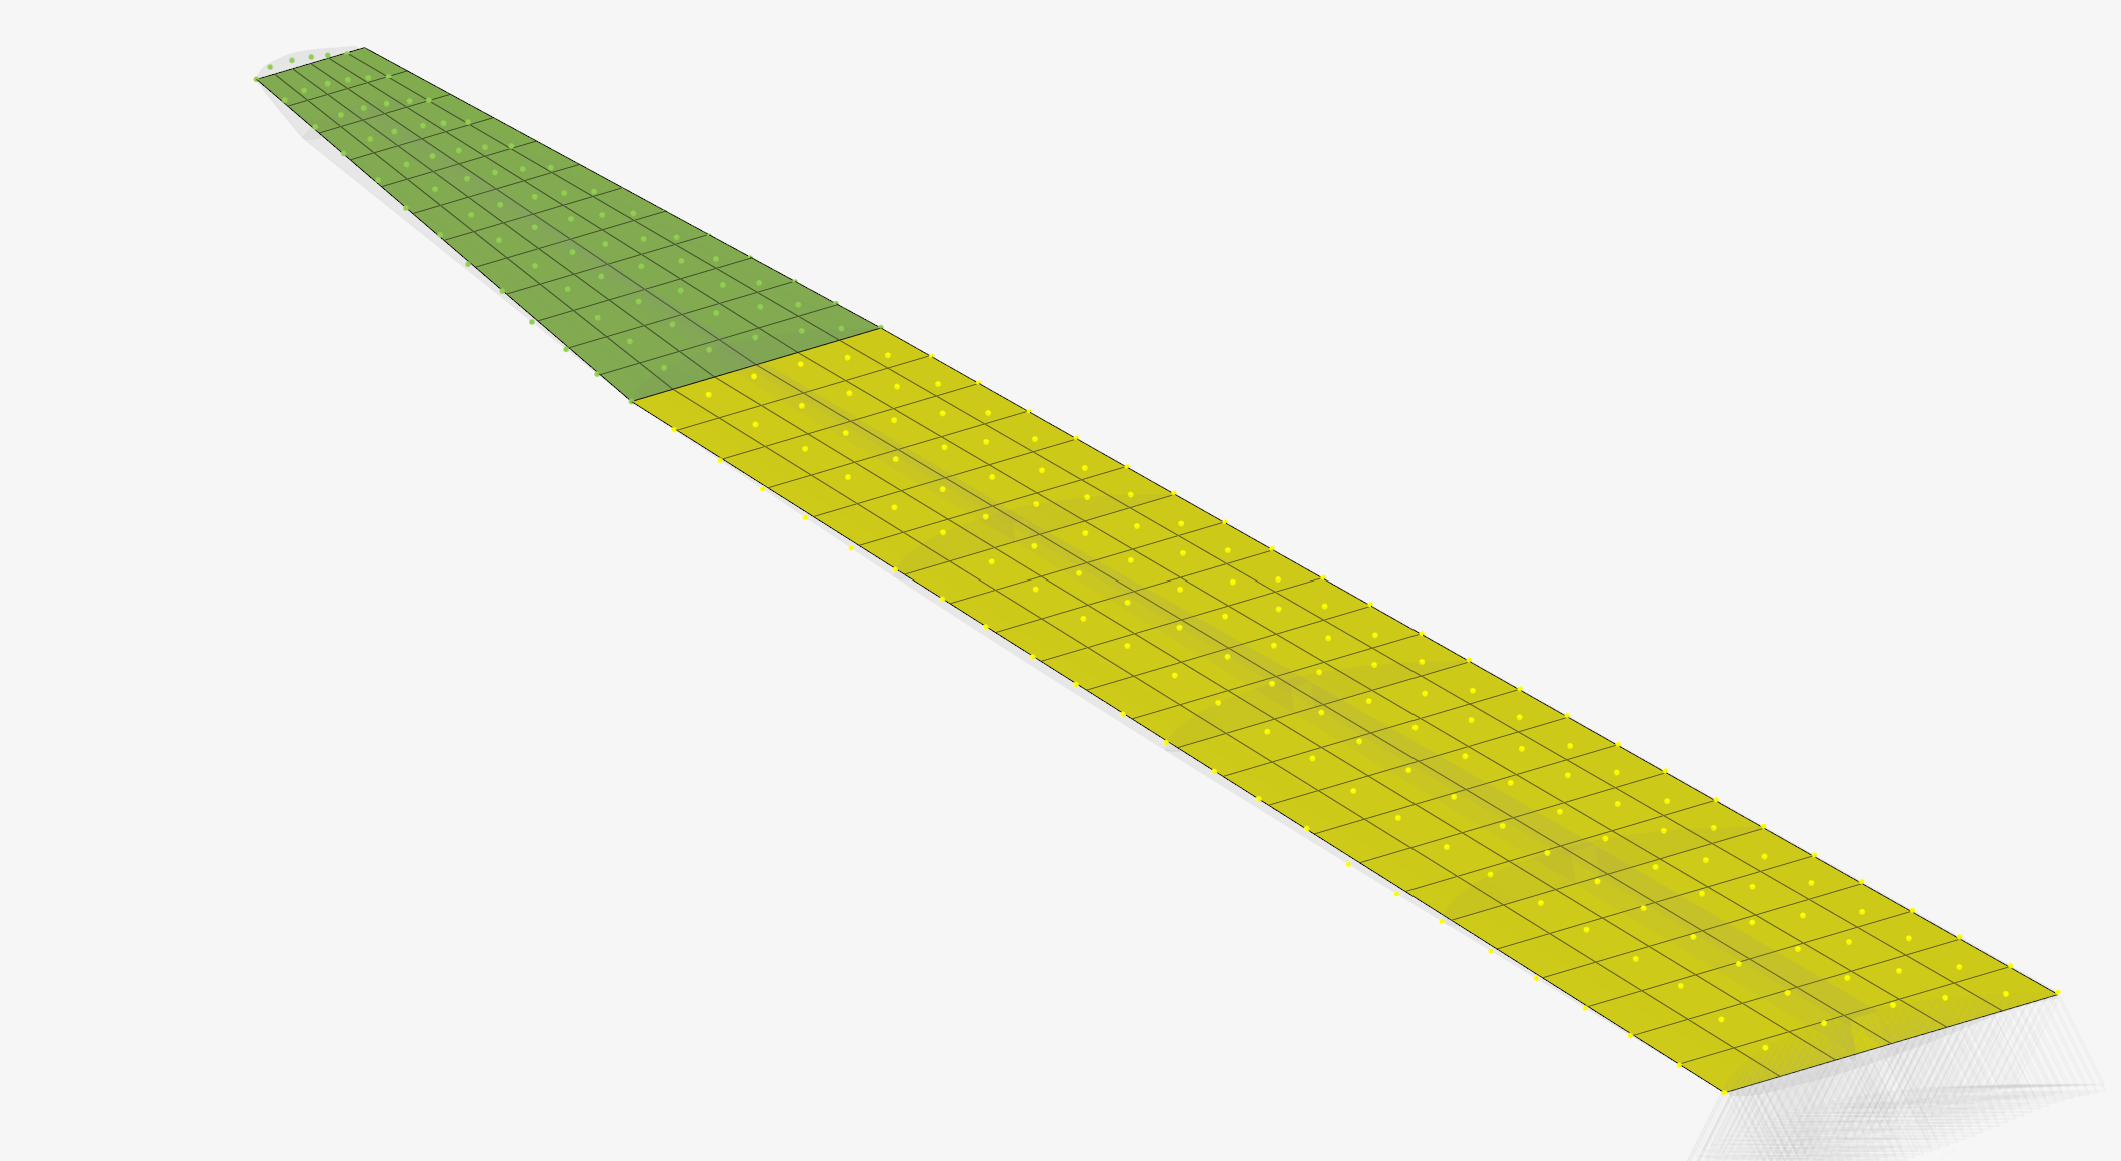
\includegraphics[width = \textwidth]{ASW 28 splines.png}
\caption{\textlatin{SPLINE1 entries} του μοντέλου της πτέρυγας \textlatin{ASW 28}}
\label{fig:SPLINE1}
\end{figure}

Όπως φαίνεται στο \autoref{fig:SPLINE1}, δημιουργήθηκαν δύο ξεχωριστά \textlatin{SPLINE1} σε αυτό το μοντέλο, μία για κάθε \textlatin{CAERO} μακρο-στοιχείο που ορίστηκε προηγουμένως. Σε αυτή την περίπτωση, επιλέγονται κόμβοι από την άνω επιφάνεια της πτέρυγας. Οι κόμβοι βρίσκονται σε σειρές κατά μήκος του άξονα της πτέρυγας σε διάφορα ποσοστά της χορδής, έτσι ώστε να ταιριάζουν καλά με τα σημεία του αεροδυναμικού πλέγματος.


\subsection{\textlatin{Setup} Αεροελαστικού προβλήματος στο \textlatin{Optistruct}} 
\label{aeroelastic-problem-setup}

Για το στήσιμο της ανάλυσης πτερυγισμού, πρέπει να οριστούν αρκετές παράμετροι.

\subsubsection{\textlatin{The AERO card:}}

Η κάρτα δεδομένων \textlatin{AERO} ορίζει βασικές παραμέτρους για την δυναμική αεροελαστικότητα που αφορούν κυρίως τις συνθήκες πτήσης. Οι εγγραφές αυτής της κάρτας συνοψίζονται ως εξής:

\begin{itemize}
\item
\textlatin{\textbf{VELOCITY}}: δεν έχει επίδραση στην ανάλυση \textlatin{Flutter}, καθώς η ταχύτητα μεταβάλλεται κατά τη διάρκεια της ανάλυσης και ορίζεται αλλού, αλλά δεν μπορεί να αφεθεί κενή, οπότε εισάγεται η τιμή μονάδας.
\item
\textlatin{\textbf{REFC:}} Το μήκος της χορδής αναφοράς που χρησιμοποιείται για τον υπολογισμό της μειωμένης συχνότητας και των συντελεστών ανύψωσης και αντίστασης, αν ζητηθούν, \(REFC = 0.92m\).
\item
\textlatin{\textbf{RHOREF:}} Η πυκνότητα αναφοράς \(RHOREF = 1.225\ kg\text{/}m^{3}\), η οποία είναι η πυκνότητα του αέρα στο επίπεδο της θάλασσας.
\item
\textlatin{\textbf{SYMXZ:}} Ορίζει την συμμετρία για το επίπεδο $XZ$ και μπορεί να έχει τρεις τιμές

  \begin{itemize}
  \item
    \textbf{-}1\textbf{:} για αντισυμμετρία.
  \item
    0: για καμία συμμετρία.
  \item
    1: για συμμετρία.
  \end{itemize}
\end{itemize}

\begin{quote}
Για αυτή την εφαρμογή \(SYMZX\  = 1\)
\end{quote}

\begin{itemize}
\item
\textlatin{\textbf{SYMXY:}} Ορίζει την συμμετρία για το επίπεδο $XY$ με παρόμοιο τρόπο. Στην ανάλυση αυτή \(SYMXY = 0\)
\end{itemize}

\subsubsection{\textlatin{The MKAERO1 card:}}

Η κάρτα \textlatin{MKAERO1} είναι μια \textlatin{bulk data entry} κάρτα που χρησιμοποιείται για την εισαγωγή ενός πίνακα αριθμών \textlatin{Mach} και μειωμένων συχνοτήτων για τις οποίες υπολογίζονται οι αεροδυναμικοί πίνακες.

Η μορφή της κάρτας \textlatin{MKAERO1} έχει δύο στήλες με μέγιστο αριθμό οκτώ στοιχείων η καθεμία. Η μία στήλη είναι για την εισαγωγή του αριθμού \textlatin{Mach}, ενώ η άλλη για τις μειωμένες συχνότητες. Οι αεροδυναμικοί πίνακες υπολογίζονται για κάθε ζεύγος τιμών μειωμένης συχνότητας και αριθμού \textlatin{Mach}.

Δεν υπάρχουν συγκεκριμένες συστάσεις για το εύρος των μειωμένων συχνοτήτων που πρέπει να καλύπτονται από αυτήν την κάρτα, αλλά καθώς γίνεται παρεμβολή μεταξύ των αεροδυναμικών πινάκων στην πραγματική τελική μειωμένη συχνότητα, η λογική υποδεικνύει ότι το εύρος των μειωμένων συχνοτήτων πρέπει να είναι τουλάχιστον μεγαλύτερο από το αποτέλεσμα του εύρους των μειωμένων συχνοτήτων. Φυσικά, αυτό δεν μπορούμε να το γνωρίζουμε εκ των προτέρων, καθώς οι τελικές μειωμένες συχνότητες καθίστανται γνωστές μόνο αφού εκτελεστεί η ανάλυση. Για αυτή την ανάλυση χρησιμοποιήθηκε ένα μεγάλο εύρος μειωμένων συχνοτήτων όπως προτάθηκε από πολλά παρόμοια παραδείγματα αυτού του τύπου ανάλυσης.

Σε περίπτωση που απαιτούνται περισσότερες από οκτώ τιμές για τη μειωμένη συχνότητα ή τον αριθμό \textlatin{Mach}, μπορεί να εισχθεί μια δεύτερη κάρτα \textlatin{MKAERO1}.

Οι τιμές που χρησιμοποιήθηκαν είναι οι εξής:

\[\overrightarrow{M} = \begin{matrix}
0.0
\end{matrix},\ \ \overrightarrow{K} = \begin{bmatrix}
0.2 \\
0.4 \\
0.8 \\
1.6 \\
3.2 \\
6.4 \\
10 \\
14
\end{bmatrix}\]

Όπως φαίνεται, υπάρχει μόνο ένας αριθμός \textlatin{Mach} \(M = 0\), που σημαίνει ότι υποθέτουμε ασυμπίεστο ρευστό. Οι αεροδυναμικοί πίνακες υπολογίζονται σε κάθε σημείο \(\left( M_{i}, K_{j} \right)\)

\subsubsection{\textlatin{The FLFACT card:}}

Η κάρτα δεδομένων bulk \textlatin{bulk FLFACT} είναι μια κάρτα που καθορίζει μια σειρά αεροδυναμικών παραμέτρων. Αυτές οι παράμετροι χρησιμοποιούνται για να ορίσουν:

\begin{enumerate}
\def\labelenumi{\arabic{enumi}.}
\item
  Τις αναλογίες πυκνότητας.
\item
  Τους αριθμούς \textlatin{Mach}.
\item
  Τις μειωμένες συχνότητες ή ταχύτητες (μόνο για την μέθοδο $PK$).
\end{enumerate}

Αυτοί οι παράγοντες μπορούν να οριστούν χρησιμοποιώντας δύο διαφορετικές μορφές.

\begin{enumerate}
\def\labelenumi{\arabic{enumi}.}
\item
  Στη Μορφή 1, μια σειρά τιμών εισάγεται απευθείας στην κάρτα.
\item
  Στη Μορφή 2 χρησιμοποιείται η λεγόμενη μορφή \textlatin{THRU} για τον ορισμό μιας σειράς τιμών, χρησιμοποιώντας:

  \begin{enumerate}
  \def\labelenumii{\alph{enumii}.}
  \item
    $F1$: Ο πρώτος παράγοντας.
  \item
    $FNF$: Ο τελικός παράγοντας.
  \item
    $NF$: Ο αριθμός των παραμέτρων (ακέραιος).
  \item
    $FMID$: Ο ενδιάμεσος αεροδυναμικός παράγοντας.
  \end{enumerate}
\end{enumerate}

Η πραγματική σειρά τιμών που παράγεται όταν χρησιμοποιείται η μορφή \textlatin{THRU} υπολογίζεται χρησιμοποιώντας τον παρακάτω τύπο:


\begin{multline}
\frac{F1(FNF - FMID)(NF - i) + FNF(FMID - F1)(i - 1)}{(FNF - FMID)(NF - i) + (FMID - F1)(i - 1)}\\ , \text{Όπου }\ i = 1,2\ldots,NF
\end{multline}

Σημειωτέον ότι όταν \(FMID = \frac{F1 + FNF}{2}\) οι παράγοντες κατανέμονται εξίσου μεταξύ \(F1\) και \(FNF\).

Για αυτήν την ανάλυση απαιτούνται τρεις κάρτες \textlatin{FLFACT}:

\begin{itemize}
\item
  \textlatin{\textbf{FLFACT 1}}: Είναι ο συντελεστής πυκνότητας και έχει τιμή \(1\). Αυτός ο συντελεστής είναι πολλαπλασιαστής της αναφορικής πυκνότητας που ορίζεται στην κάρτα \textlatin{AERO} και υποδεικνύει ότι η ανάλυση θα εκτελεστεί με πυκνότητα \(1 \times RHOREF\).
\item
  \textlatin{\textbf{FLFACT 2}}: Είναι ο αριθμός \textlatin{Mach} και έχει τιμή \(0\). Αυτός ο συντελεστής είναι ο αριθμός \textlatin{Mach} στον οποίο θα εκτελεστεί η ανάλυση .
\item
  \textlatin{\textbf{FLFACT 3}}: Είναι η ταχύτητα/ες στις οποίες θα εκτελεστεί η ανάλυση . Αυτή η \textlatin{FLFACT} ορίζεται χρησιμοποιώντας τη Μορφή \textlatin{THRU} με παράγοντες:

  \begin{itemize}
  \item
    \(F1 = 20m/s\)
  \item
    \(FNF = 320m/s\)
  \item
    \(NF = 30\)
  \item
    \(FMID = 160\)
  \end{itemize}
\end{itemize}

Η ανάλυση εκτελείται για κάθε συνδυασμό πυκνότητας, αριθμού \textlatin{Mach} και ταχύτητας στις κάρτες \textlatin{FLFACT}.

\subsubsection{\textlatin{The Flutter card:}}

Η \textlatin{bulk data entry card Flutter}  καθορίζει τη μέθοδο και τις παραμέτρους της αεροελαστικής ανάλυσης πτερυγισμού:

Τα πιο σημαντικά πεδία αυτής της κάρτας είναι:

\begin{enumerate}
\def\labelenumi{\arabic{enumi}.}
\item
\textlatin{\textbf{METHOD}}: Η μέθοδος μπορεί να είναι μία από τις $K$, $PK$, $PKNL$, $KE$. Για αυτήν την ανάλυση χρησιμοποιείται η μέθοδος $PK$.
\item
\textlatin{\textbf{DENS}}: Αναφορά στην κάρτα δεδομένων \textlatin{FLFACT} που καθορίζει τους πολλαπλασιαστές πυκνότητας.
\item
\textlatin{\textbf{MACH}}: Αναφορά στην κάρτα δεδομένων \textlatin{FLFACT} που καθορίζει τον αριθμό \textlatin{Mach}.
\item
\textlatin{\textbf{VEL}}: Αναφορά στην κάρτα δεδομένων \textlatin{FLFACT} που καθορίζει τις ταχύτητες.
\item
\textlatin{\textbf{IMETH}}: Η μέθοδος παρεμβολής για τον αεροδυναμικό πίνακα, η οποία μπορεί να είναι είτε L είτε S για γραμμική ή επιφανειακή παρεμβολή αντίστοιχα. Η προεπιλεγμένη τιμή L διατηρείται για αυτήν την ανάλυση.
\end{enumerate}

\subsubsection{\textlatin{The EIGRL card:}}

Η  \textlatin{bulk data entry card EIGRL} ορίζει τα δεδομένα που απαιτούνται για την εκτέλεση ανάλυσης πραγματικών ιδιοτιμών με τη μέθοδο \textlatin{Lanczos}. Τα κύρια πεδία αυτής της κάρτας είναι:

\begin{enumerate}
\def\labelenumi{\arabic{enumi}.}
\item
  $V1$, $V2$ Εύρος συχνοτήτων της ανάλυσης.
\item
  $ND$ Αριθμός επιθυμητών ιδιοσυχνοτήτων.
\end{enumerate}

Για αυτήν την ανάλυση, χρησιμοποιούνται οι τιμές \(V1 = 0.0\ Hz\) και \(ND = 8\).
Αυτές οι τιμές σημαίνουν ότι θα υπολογιστούν οι πρώτες οκτώ ιδιοσυχνότητες ξεκινώντας από $0 Hz$.



\subsubsection{\textlatin{Subcase Definition:}}

Για τον ορισμό του \textlatin{subcase}, επιλέγεται ο τύπος ανάλυσης \textlatin{ ``Aeroelastic Flutter''} και στη συνέχεια:

\begin{itemize}
\item
  Το πεδίο \textlatin{FMETHOD} απαιτεί αναφορά στην κάρτα \textlatin{Flutter}.
\item
  Το πεδίο \textlatin{SPC} απαιτεί αναφορά στον \textlatin{load collector SPC}.
\item
  Το πεδίο \textlatin{METHOD} απαιτεί αναφορά στο \textlatin{EIGRL}.
\item
  Το πεδίο \textlatin{CMETHOD} απαιτεί αναφορά σε μια κάρτα \textlatin{EIGC} αλλά μπορεί να παραμείνει κενό αν δεν χρειάζεται να υπολογιστούν σύνθετες ιδιοτιμές (είναι κενό σε αυτή την περίπτωση καθώς δεν λαμβάνεται υπόψη η δομική απόσβεση).
\item
  Το πεδίο \textlatin{SMETHOD} απαιτεί αναφορά σε καμπύλη απόσβεσης \textlatin{TDMP} αλλά μπορεί να παραμείνει κενό εφ'όσον δεν λαμβάνεται υπόψη η δομική απόσβεση (είναι κενό σε αυτή την περίπτωση καθώς δεν λαμβάνεται υπόψη η δομική απόσβεση).
\end{itemize}

Τα αποτελέσματα της αεροελαστικής ανάλυσης πτερυγισμού παρουσιάζονται στην \autoref{initial-flutter-analysis}.

\section{\textlatin{Optistruct} -- Διεπαφή με \textlatin{Python}}
\label{optistruct-python-interface}

\subsection{Αποτελέσματα Ανάλυσης Πτερυγισμού \&\ \textlatin{Python} }
\label{results-of-flutter-analysis-python}

Η έξοδος της ανάλυσης που ορίζεται στην προηγούμενη ενότητα είναι ένα αρχείο κειμένου \textlatin{.flt} εκτός από το τυπικό αρχείο εξόδου \textlatin{.out} του \textlatin{Optistruct}. Έχει πολύ συγκεκριμένη μορφή. Είναι οργανωμένο σε μπλοκ πληροφοριών, κάθε ένα από τα οποία αντιστοιχεί σε ένα διαφορετικό συνδυασμό αριθμού \textlatin{Mach}, \textlatin{πυκνότητας} (ορισμένα στις κάρτες \textlatin{FLFACT}) και αριθμού ιδιομορφής. Τα πιο σημαντικά χαρακτηριστικά του αρχείου \textlatin{.flt} περογράφονται στο \autoref{fig:Optistruct.fltfileexplanation}.


\begin{figure}[H]
    \centering
    \includesvg[width=\textwidth]{Flt file explanation.svg}
    \caption{Επεξήγηση του \textlatin{Optistruct .flt file}}
    \label{fig:Optistruct.fltfileexplanation}
\end{figure}

Το τυπικό αρχείο \textlatin{.out}, το οποίο επίσης εξάγεται, περιέχει πληροφορίες σχετικά με το αν ο επιλυτής ενέπεσε σε σφάλμα ή προειδοποιήσεις και, το πιο σημαντικό, πληροφορίες σχετικά με τη μάζα του μοντέλου.

Από τα δεδομένα που περιέχονται στο αρχείο \textlatin{.flt}, μπορούν να παραχθούν δύο πολύ χρήσιμα διαγράμματα. 


\begin{enumerate}
  \def\labelenumi{\arabic{enumi}.}
  \item
    Το διάγραμμα $V-g$ απεικονίζει την απόσβεση κάθε ιδιομορφής (άξονας $y$) ως προς την Ταχύτητα (άξονας $x$).
  \item
    Το διάγραμμα $V-f$ απεικονίζει τη συχνότητα κάθε ιδιομορφής (άξονας $y$) ως προς την Ταχύτητα (άξονας $x$).
\end{enumerate}
  
Ένα τυπικό παράδειγμα αυτών τον διαγραμμάτων φαίνεται στο \autoref{fig:VGVFexapleplot} 

\begin{figure}[H]
  \centering
  \begin{minipage}{0.495\textwidth}
      \centering
      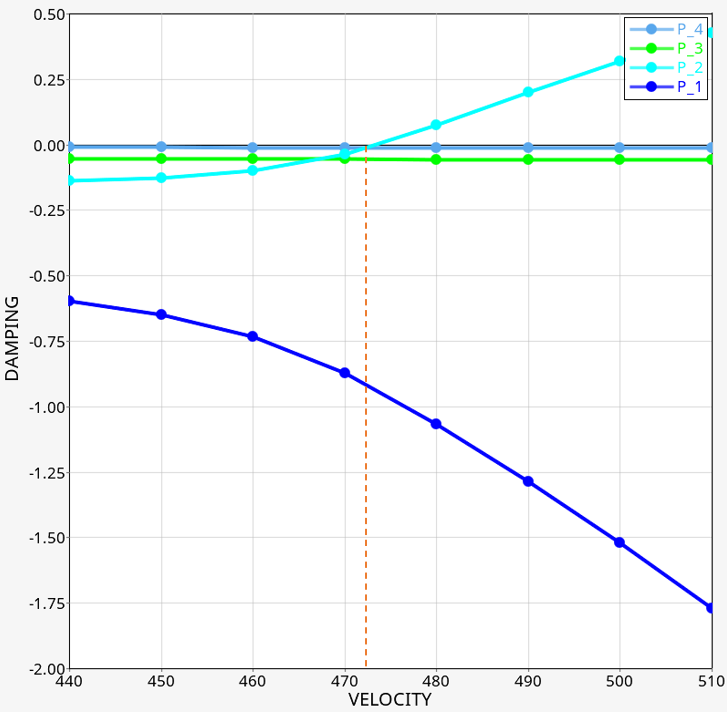
\includegraphics[width=\linewidth]{Example VG plot.png}
  \end{minipage}
  \hfill
  \begin{minipage}{0.495\textwidth}
      \centering
      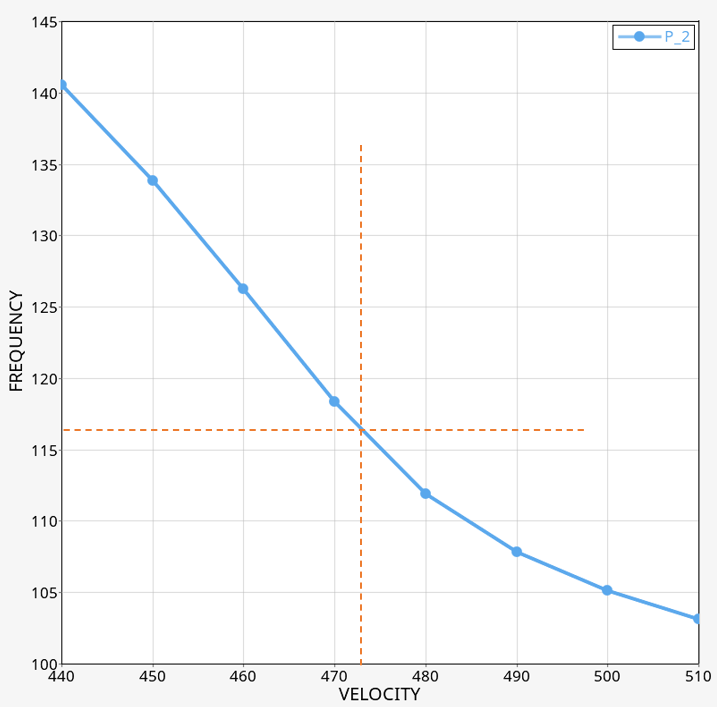
\includegraphics[width=\linewidth]{Example VF plot.png}

  \end{minipage}
  \caption{Παραδείγματα απο \textlatin{V-g}  και \textlatin{V-f plots} με τέσσερις ιδιομορφές \cite{altair_flutter_tips}}
  \label{fig:VGVFexapleplot}
\end{figure}


Από αυτά τα δεδομένα μπορεί να προσδιοριστεί η ταχύτητα πτερυγισμού εξετάζοντας το διάγραμμα $V-g$. Πιο συγκεκριμένα, μια ιδιομορφή αποκλίνει όταν η απόσβεσή της γίνεται από αρνητική, θετική. Πολλές ιδιομορφές μπορεί να αποκλίνουν, αλλά η ταχύτητα πτερυγισμού του μποντέλου προσδιορίζεται από την ιδιομορφή που αποκλίνει στη χαμηλότερη ταχύτητα.

Τα δεδομένα που περιέχονται στο αρχείο \textlatin{.flt} διαβάζονται από ένα πρόγραμμα \textlatin{Python} και αποθηκεύονται ως \textlatin{pandas data frames}. Για να προσδιοριστεί η ταχύτητα πτερυγισμού, παρακολουθούνται οι αλλαγές του προσήματος της απόσβεσης κάθε ιδιομορφής μέχρι να ανιχνευτεί μια αλλαγή από αρνητικό σε θετικό πρόσημο. Στη συνέχεια, καταγράφονται όλα τα σημεία όπου παρατηρείται τέτοια αλλαγή και η ταχύτητα πτερυγισμού προσδιορίζεται από την ελάχιστη ταχύτητα στην οποία συμβαίνει αυτή η αλλαγή.

Μια άλλη συνάρτηση είναι υπεύθυνη για την ανάγνωση του αρχείου \textlatin{.out} από όπου καθορίζεται αν ο επιλυτής ολοκλήρωσε την ανάλυση με επιτυχία καθώς και τη μάζας του μοντέλου.

\subsection{Τροποποίηση της εισόδου του \textlatin{Optistruct} χρησιμοποιώντας \textlatin{Python}}
\label{modifying-optistructs-input-using-python}

Για να γίνει βελτιστοποίηση του σύνθετου υλικού της πτέρυγας, είναι απαραίτητο να τροποποιηθούν οι ιδιοτήτες του σύνθετου υλικού προγραμματιστικά, έτσι ώστε να δοκιμαστούν πολλές διαφορετικές παραλλαγές και να φτάσουμε σε μια βέλτιστη λύση. Το \textlatin{Optistruct} διευκολύνει αυτή τη διαδικασία αρκετά, διότι χρησιμοποιεί ένα αρχείο κειμένου για είσοδο, που κωδικοποιεί όλες τις πληροφορίες του μοντέλου. Αυτό το αρχείο ονομάζεται \textlatin{.fem} και μπορεί να εξαχθεί από το \textlatin{HyperMesh} με μορφή \textlatin{csv}. Για να τροποποιηθούν οι ιδιότητες του σύνθετου υλικού, εντοπίζεται το σωστό τμήμα αυτού του αρχείου και αποκωδικοποιείται. Σύμφωνα με το εγχειρίδιο του \textlatin{Optistruct}, οι ιδιότητες του σύνθετου υλικού κωδικοποιούνται με τον τρόπο που φαίνεται στον \autoref{tab:OptistructPCOMPcard}.


\begin{table}[h]
  \centering
  \resizebox{\linewidth}{!}{ % Fits table to page width
    \begin{tabular}{|c|c|c|c|c|c|c|c|c|c|}
      \hline
      1 & 2 & 3 & 4 & 5 & 6 & 7 & 8 & 9 & 10 \\ 
      \hline
      $PCOMP$ & $PID$ & $Z0$ & $NSM$ & $SB$ & $FT$ & $TREF$ & $GE$ & $LAM$ & $+$ \\ 
      \hline
      & $MID1$ & $T1$ & $THETA1$ & $SOUT1$ & $MID2$ & $T2$ & $THETA2$ & $SOUT2$ & $+$ \\ 
      \hline
      & $MID3$ & $T3$ & $THETA3$ & $SOUT3$ & $Etc.$ & & & & \\ 
      \hline
    \end{tabular}
  }
  \caption{H \textlatin{bulk data entry} κάρτα \textlatin{PCOMP} του \textlatin{Optistruct}}
  \label{tab:OptistructPCOMPcard}
\end{table}


Όπου:

\begin{itemize}
  \item
    $PCOMP$: είναι η λέξη-κλειδί που υποδεικνύει ότι ακολουθεί ορισμός ιδιοτήτων σύνθετου υλικού \textlatin{(string)}.
  \item
    $PID$: είναι το ID της ιδιότητας \textlatin{(integer)}.
  \item
    $NSM$: είναι η μη-δομική μάζα ανά μονάδα επιφάνειας \textlatin{(float)}.
  \item
    $SB$: επιτρεπτό μέγιστο τόξο ενδο-στρώματος \textlatin{(default 0.0) (float)}.
  \item
    $FT$: Επιλογή θεωρίας αστοχίας.
  \item
    $TREF$: Θερμοκρασία χωρίς τάση \textlatin{(float)}.
  \item
    $GE$: Συντελεστής απόσβεσης \textlatin{(float)}.
  \item
    $LAM$: Επιλογή \textlatin{laminate}, διάφοροι τρόποι ορισμού του \textlatin{laminate}. Στην προεπιλεγμένη περίπτωση, όλα τα \textlatin{plies} πρέπει να οριστούν ένα προς ένα.
  \item
    $MIDi$: Το \textlatin{ID} του υλικού του \textlatin{ply i} \textlatin{(integer)}.
  \item
    $Ti$: Το πάχος του \textlatin{ply i}.
  \item
    $THETAi$: Η γωνία του \textlatin{ply i}.
  \item
    $SOUTi$: Αίτημα εξόδου τάσης, παραμόρφωσης, \textlatin{default False, (bool)}.
\end{itemize}
  

Οι μεταβλητές που πρέπει να τροποποιηθούν είναι κυρίως οι $Ti$ και $THETAi$.

\section{Πρόβλημα Βελτιστοποίησης}\label{optimization-problem}

Σε αυτή την ενότητα θα συζητηθεί η εφαρμογή των αλγορίθμων βελτιστοποίησης που αναφέρθηκαν στην \autoref{optimization-techniques}.

\subsection{Εφαρμογή της Μεθόδου \textlatin{Powell}}
\label{applying-powells-method}

Αυτός ο αλγόριθμος υλοποιήθηκε χρησιμοποιώντας τη συνάρτηση \textlatin{minimize} της $SciPy$ \cite{2020SciPy-NMeth} επιλέγοντας την προαιρετική παράμετρο \textlatin{\emph{method = ``Powell''}}.
Για να οριστεί πλήρως το πρόβλημα βελτιστοποίησης, πρέπει να οριστούν και μερικές ακόμα συμαντικές παράμετροι.

\subsubsection{Μεταβλητές Απόφασης:}

Το πρώτο βήμα είναι ο ορισμός των μεταβλητών απόφασης. Αυτές οι μεταβλητές είναι το πάχος και η γωνία κάθε στρώσης \textlatin{ply} του σύνθετου υλικού. Επειδή το \textlatin{laminate} αποτελείται από έξι στρώσεις, αυτό σημαίνει ότι θα πρέπει να χρησιμοποιηθούν 12 μεταβλητές απόφασης.

Λόγω του υπολογιστικού χρόνου που απαιτείται, πρέπει να γίνουν κάποιες υποθέσεις για να μειωθεί η πολυπλοκότητα του προβλήματος βελτιστοποίησης. Αυτές οι υποθέσεις είναι:


\begin{itemize}
  \item
    Οι στρώσεις είναι αντισυμμετρικές.
  
  Αυτό σημαίνει ότι για κάθε στρώση σε ύψος \(z_{k}\) με γωνία \(\theta_{k}\) πάνω από τη μεσαία επιφάνεια, υπάρχει μια αντίστοιχη στρώση με αντίθετη γωνία  \(- \theta_{k}\) σε ύψος \(- z_{k}\) από τη μεσαία επιφάνεια, όπως φαίνεται στο \autoref{fig:Antisymmetric layer configuration} 

  

\begin{figure}[H]
    \centering
    \includesvg[width=0.7\textwidth]{Antisymmetric layers.svg}
    \caption{Αντισυμμετρικά στρώματα σύνθετου υλικού}
    \label{fig:Antisymmetric layer configuration}
    
\end{figure}


Αυτή η υπόθεση μειώνει τον αριθμό των μεταβλητών απόφασης για τις γωνίες στρώσης στο μισό, διότι από τις αρχικές έξι ανεξάρτητες μεταβλητές, μόνο τρεις χρειάζεται να οριστούν για το \textlatin{laminate} έξι στρώσεων \([ \theta_{1},\ \ \theta_{2},\ \ \theta_{3}]\) .

Αυτή η υπόθεση είναι λογική, καθώς τα περισσότερα σύνθετα υλικά είναι είτε συμμετρικά είτε αντισυμμετρικά προκειμένου να μειώσουν την επίδραση του \textlatin{membrane - bending coupling}.

\item
  Κάθε στρώση έχει το ίδιο πάχος.

Αυτή η υπόθεση μειώνει τον αριθμό των ανεξάρτητων μεταβλητών από έξι σε μία, αφού μόνο ένα πάχος \([t]\) χρειάζεται να οριστεί.

Αυτή η υπόθεση είναι επίσης αρκετά λογική, καθώς κατά την κατασκευή σύνθετων μελών, κάθε στρώση προέρχεται από τον ίδιο ρολό ανθρακονήματος, το οποίο έχει ομοιόμορφο πάχος σε όλη του την επιφάνεια.
\end{itemize}


Αυτές οι δύο υποθέσεις οδηγούν στις τελικές μεταβλητές απόφασης που είναι:

\begin{equation}
\vec{\mathbf{x}}=[t,\theta_{1},\theta_{2},\theta_{3}]^{T}
\label{eq:descisionvars}
\end{equation}
\subsubsection{Αντικειμενική Συνάρτηση:}

Στη συνέχεια ορίζεται η αντικειμενική συνάρτηση. Εξετάστηκαν δύο διαφορετικές περιπτώσεις για αυτή τη συνάρτηση.

\begin{itemize}
\item
  \textbf{Περίπτωση 1}: Η συνάρτηση στόχου εξετάζει τόσο τη μάζα όσο και την ταχύτητα πτερυγισμού. Η ιδέα πίσω από τον ορισμό αυτής της αντικειμενικής συνάρτησης  είναι, να είναι δυνατός ο περιορισμός της μάζας της κατασκευής ενώ διατηρείται μια επαρκής ταχύτητα πτερυγισμού. Αυτό κανονικά θα ανήκε στην κατηγορία της πολυδιάστατης βελτιστοποίησης αλλά η μέθοδος \textlatin{Powell} δεν έχει αυτή τη δυνατότητα, οπότε χρησιμοποιείται μια εναλλακτική λύση. Η μέθοδος ποινής πρέπει να εφαρμοστεί, οδηγώντας έτσι στον εξής ορισμό.


\begin{equation}
    f_{obj}\left( \vec{\mathbf{x}} \right) =
    \begin{cases} 
        M, & V_{flutter} > V_{limit} \\
        M + P \cdot \left( V_{limit} - V_{flutter} \right), & V_{flutter} < V_{limit}
    \end{cases}
    \label{eq:objpowell1}
\end{equation}

\begin{quote}
Όπου:
\end{quote}

\begin{itemize}
  \item
    \(M\): είναι η μάζα.
  \item
    \(P\): είναι μια μεγάλη σταθερά που ονομάζεται ποινή \textlatin{(Penalty)}.
  \item
    \(V_{limit}\): είναι το όριο κάτω από το οποίο η ταχύτητα πτερυγισμού της πτέρυγας θεωρείται ανεπίτρεπτα χαμηλή.
  \item
    \(V_{flutter}\): είναι η ταχύτητα πτερυγισμού που προκύπτει από το \latintext{Optistruct}.
  \end{itemize}
  
  Αυτός ο ορισμός επιτρέπει την ελαχιστοποίηση της μάζας εξασφαλίζονατας οτι η ταχύτητα πτερυγισμού παραμένει πάνω από ένα ορισμένο όριο. Εάν η ταχύτητα πτερυγισμού πέσει κάτω από το καθορισμένο όριο, προστίθεται ένας όρος ποινής ανάλογος με την ποσότητα με την οποία παραβιάζεται ο περιορισμός, έτσι ώστε ο αλγόριθμος βελτιστοποίησης να αναγκαστεί να επιστρέψει σε μια περιοχή όπου ο περιορισμός δεν παραβιάζεται.
  

  \item
  \textbf{Περίπτωση 2}: Το απλούστερο σενάριο είναι μια αντικειμενική συνάρτηση όπου η είσοδος είναι το διάνυσμα μεταβλητών απόφασης από την εξίσωση \eqref{eq:descisionvars}, χωρίς το πάχος \(t\), και η έξοδος είναι η αρνητική ταχύτητα πτερυγισμού που υπολογίζεται από το \textlatin{Optistruct}.

\end{itemize}

\begin{equation}
f_{obj}\left( \vec{\mathbf{x}} \right) = - V_{flutter},\ \ \text{με}\ \vec{\mathbf{x}}\mathbf{=}\left\lbrack \theta_{1},\theta_{2},\theta_{3} \right\rbrack^{T}
\label{eq:objpowell2}
\end{equation}

Το αρνητικό πρόσημο στην ταχύτητα είναι απαραίτητο για να γίνει η ελαχιστοποίηση προς την κατεύθυνση της αύξησης της ταχύτητας πτερυγισμού. Εφόσον η μάζα δεν εξετάζεται στην αντικειμενική συνάρτηση, ο αλγόριθμος βελτιστοποίησης θα μπορούσε απλώς να αυξήσει το πάχος του υλικού και να επιτύχει υψηλότερη ταχύτητα πτερυγισμού. Αυτή η συμπεριφορά είναι φυσικά ανεπιθύμητη και είναι ο λόγος που το πάχος αφαιρέθηκε από τις μεταβλητές βελτιστοποίησης και τώρα παραμένει σταθερό καθ' όλη τη διάρκεια της βελτιστοποίησης, μαζί με τη μάζα της πτέρυγας.


\subsubsection{\textlatin{Search Space Boundaries}}

Για να οριστεί πλήρως το πρόβλημα βελτιστοποίησης, πρέπει να οριστεί και ο χώρος αναζήτησης. Ο ορισμός των ορίων είναι αρκετά απλός σε αυτήν την περίπτωση.

\begin{itemize}
\item
  \textbf{Για την Περίπτωση 1:} \\
  Το πάχος και οι γωνίες πρέπει να περιορισθούν. Τα όρια για το πάχος ορίζονται να είναι εντός ενός λογικού εύρους από $0.1$ έως $1 mm$ ενώ για τις γωνίες περιορίζονται μεταξύ -90 και +90 μοιρών.

  \begin{equation}
    t \in [ 10^{- 4},\ 10^{- 3} ]\quad and \quad \theta_{1},\theta_{2},\theta_{3} \in [ - 90^{o}, + 90^{o} ]
    \end{equation}


\item
  \textbf{Για την Περίπτωση 2:} \\
  Μόνο οι γωνίες πρέπει να περιορίζονται μεταξύ -90 και +90 μοιρών, οπότε οι περιορισμοί είναι:

  \begin{equation}
    \theta_{1},\theta_{2},\theta_{3} \in [ - 90^{o}, + 90^{o} ]
  \end{equation}



\end{itemize}



\subsubsection{Επιτάχυνση του αλγορίθμου}

Λόγω της υπολογιστικά εντατικής φύσης της αντικειμενικής συνάρτησης, εφαρμόστηκε μια μέθοδος για τη μείωση του υπολογιστικού χρόνου. Αντί ο αλγόριθμος να μπορεί να επιλέξει οποιονδήποτε αυθαίρετο πραγματικό αριθμό εντός του καθορισμένου εύρους κάθε μεταβλητής βελτιστοποίησης, βρέθηκε μια συμβιβαστική λύση. Οι τιμές κάθε μεταβλητής στρογγυλοποιούνται εσωτερικά σε μια καθορισμένη ακρίβεια που δίνεται από τον χρήστη. Επιπλέον, τα αποτελέσματα κάθε επανάληψης αποθηκεύονται σε μνήμη \textlatin{cache} έτσι ώστε σε περίπτωση που ο αλγόριθμος προσπαθήσει να χρησιμοποιήσει την ίδια είσοδο, οι υπολογισμοί να παραλείπονται και αντ'αυτών να χρησιμοποιούνται τα αποθηκευμένα αποτελέσματα. Η αποθήκευση στην \textlatin{cache} σε συνδυασμό με τη στρογγυλοποίηση οδηγεί σε πολύ λιγότερες κλήσεις στον επιλυτή \textlatin{Optistruct} από ό,τι θα απαιτούνταν διαφορετικά. Για την εφαρμογή αυτή, οι γωνίες στρογγυλοποιούνται στον πλησιέστερο ακέραιο, ενώ το πάχος στρογγυλοποιείται στο πλησιέστερο δέκατο του χιλιοστού.

Για να γίνει πιο σαφής αυτή η έννοια, ακολουθεί ένα παράδειγμα: \\


Ας υποθέσουμε ότι το αρχικό διάνυσμα είναι
\({\vec{x}}_{0} = \lbrack 0.0005,\ \ 45,\  - 45,\ 45\rbrack^{T}\)

\begin{enumerate}
\def\labelenumi{\arabic{enumi}.}
\item
  Για την πρώτη επανάληψη ας υποθέσουμε ότι ο αλγόριθμος προσπαθεί

\[{\vec{x}}_{1} = \lbrack 0.00043,\  - 20.3,\  - 69.6\ ,\ 42.14\rbrack^{T}\]

αυτό θα στρογγυλοποιηθεί εσωτερικά σε

\[{\vec{x}}_{1} = \lbrack 0.0004,\ \ 20,\  - 70,\ 42\rbrack^{T}\]

και το αποτέλεσμα θα αποθηκευτεί στην \textlatin{cache}

\item
  Αν στη δεύτερη επανάληψη ο αλγόριθμος προσπαθήσει

\[{\vec{x}}_{2} = \lbrack 0.00041,\  - 20.4,\  - 69.8\ ,\ 42.47\rbrack^{T}\]

θα στρογγυλοποιηθεί και αυτό σε

\[{\vec{x}}_{2} = \lbrack 0.0004,\ \ 20,\  - 70,\ 42\rbrack^{T}\]

και το ίδιο αποθηκευμένο αποτέλεσμα θα χρησιμοποιηθεί.
\end{enumerate}


Τα αποτελέσματα της μεθόδου \textlatin{Powell} παρουσιάζονται στην \autoref{powells-optimization-method}



\subsection{Εφαρμογή του Γενετικού Αλγορίθμου}
\label{applying-the-genetic-algorithm}

Για την εφαρμογή του γενετικού αλγορίθμου χρησιμοποιείται η βιβλιοθήκη \textlatin{PyGAD} \cite{gad2023pygad}. Για να οριστεί το πρόβλημα βελτιστοποίησης για το γενετικό αλγόριθμο, πρέπει να οριστούν πολλές παράμετροι. Δυστυχώς, δεν υπάρχει τρόπος να βρεθούν οι βέλτιστες παράμετροι για κάθε μεταβλητή σε κάθε συγκεκριμένο πρόβλημα. Επομένως, οι παράμετροι επιλέχθηκαν μετά από κάποιο πειραματισμό χρησιμοποιώντας ένα μικρότερο αριθμό γενεών που μπορούν να εκτελούνται πιο γρήγορα. Οι παράμετροι που επιλέχθηκαν πιθανότατα δεν είναι οι βέλτιστοι, αλλά λειτουργούν αρκετά καλά.

\begin{enumerate}
\def\labelenumi{\arabic{enumi}.}
\item
  Αρχικά, πρέπει να αποφασιστούν τα \textbf{γονίδια} (\textlatin{genes}) και ο \textbf{χώρος των γονιδίων} \textlatin{(gene space)}.

Τα γονίδια είναι αντίστοιχα με τις μεταβλητές βελτιστοποίησης των κλασικών αλγορίθμων βελτιστοποίησης και επιλέγονται οι τρεις γωνίες και το πάχος των στρώσεων, δηλαδή τέσσερα γονίδια συνολικά.

Ακόμη, πρέπει να οριστεί ένα εύρος δυνατών τιμών για κάθε γονίδιο. Το εύρος για κάθε γονίδιο γωνίας είναι:

\[\vartheta_{RANGE} = \lbrack - 90,\  + 90,\ \ step = 1\rbrack\]

και για το πάχος:

\[t_{RANGE} = \lbrack 0.0001,\ 0.001,\ \ step = 0.0001\rbrack\]

αυτά τα εύρη ορίζουν το χώρο των γονιδίων.

\item
  Πρέπει να οριστεί το \textlatin{fittness function} . Το \textlatin{fittness function}  είναι αντίστοιχο με την αντικειμενική συνάρτηση των κλασικών αλγορίθμων βελτιστοποίησης. Λόγω των προηγμένων δυνατοτήτων αυτού του αλγορίθμου, εκτελείται μια βελτιστοποίηση πολλαπλών στόχων , όπου οι δύο στόχοι είναι:

  \begin{itemize}
  \item
    Η ελαχιστοποίηση της μάζας της δομής του πτερυγίου \textlatin{ASW 28}.
  \item
    Η μεγιστοποίηση της ταχύτητας πτερυγισμού.
  \end{itemize}

Για να επιτευχθούν αυτοί οι στόχοι, δημιουργείται μια συνάρτηση με την εξής μορφή:

\begin{equation}
f_{fitness}\left( \begin{bmatrix}
t \\
\vartheta_{1} \\
\vartheta_{2} \\
\vartheta_{3}
\end{bmatrix} \right)\  = \begin{bmatrix}
 - Mass \\
V_{flutter}
\end{bmatrix}
\end{equation}


Το αρνητικό πρόσημο στη μάζα οφείλεται στο γεγονός ότι αυτός ο αλγόριθμος λειτουργεί με σκοπό τη μεγιστοποίηση της συνάρτησης καταλληλότητας.

\end{enumerate}

Μετά την οριστικοποίηση αυτών των βασικών και υποχρεωτικών εισόδων, ορίζονται αρκετές άλλες παράμετροι που ελέγχουν τον τρόπο λειτουργίας του αλγορίθμου.

\begin{itemize}
\item
  \textlatin{\emph{Num\_generations = 1000,}} ελέγχει τον αριθμό των γενεών στο διάστημα των οποίων θα πραγματοποιηθεί η εξέλιξη. Αυτή η παράμετρος επιλέγεται έτσι ώστε να διατηρείται ένας λογικός χρόνος υπολογισμού.
\item
\textlatin{\emph{sol\_per\_pop = 10,}} ο αριθμός των λύσεων που θα παραχθούν (ο αριθμός των χρωμοσωμάτων) μετά από κάθε γενιά.
\item
\textlatin{\emph{parent\_selection\_type = steady state selection}}
\item
\textlatin{\emph{keep\_elitisism = 4,}} που σημαίνει ότι οι τέσσερις καλύτερες λύσεις κάθε γενιάς μεταφέρονται στην επόμενη.
\item
\textlatin{\emph{crossover\_type = ``single point''}}
\item
\textlatin{\emph{crossover\_probability = 0.7,}} η πιθανότητα επιλογής ενός γονέα για την εφαρμογή της γενετικής διασταύρωσης. Για κάθε γονέα, δημιουργείται μια τυχαία τιμή μεταξύ 0.0 και 1.0. Αν αυτή η τυχαία τιμή είναι μικρότερη ή ίση με την τιμή που έχει ανατεθεί στην παράμετρο \textlatin{crossover\_probability}, τότε ο γονέας επιλέγεται.
\item
\textlatin{\emph{mutation\_type = ``random''}}
\item
\textlatin{\emph{mutation\_probability = 0.1}}, η πιθανότητα επιλογής ενός γονιδίου για την εφαρμογή της μετάλλαξης. Σε κάθε γονίδιο σε μια λύση, αναθέτεται μια τυχαία τιμή μεταξύ 0.0 και 1.0. Αν αυτή η τυχαία τιμή είναι μικρότερη ή ίση με την τιμή που έχει ανατεθεί στην παράμετρο \textlatin{mutation\_probability}, τότε το γονίδιο επιλέγεται.
\item
\textlatin{\emph{mutation\_by\_replacement = True}}, σημαίνει ότι το γονίδιο αντικαθίσταται από την τυχαία τιμή που δημιουργείται αντί να προστεθεί η μετάλαξη στην υπάρχουσα τιμή του.
\end{itemize}

Τα αποτελέσματα του Γενετικού Αλγορίθμου παρουσιάζονται στήν \autoref{genetic-algorithm-optimization}


\subsection{Πρόβλεψη Ταχύτητας πτερυγισμού μέσω Νευρωνικών Δικτύων}
\label{flutter-speed-prediction-using-neural-networks}

Ο σκοπός αυτής της ενότητας είναι η ανάπτυξη ενός υποκατάστατου μοντέλου (\textlatin{surrogate model}) χρησιμοποιώντας Νευρωνικά Δίκτυα για να επιταχυνθεί η διαδικασία της βελτιστοποίησης. Τα υποκατάστατα μοντέλα χρησιμοποιούνται συχνά στη μηχανική όταν το αποτέλεσμα που μας ενδιαφέρει δεν μπορεί να μετρηθεί εύκολα ή όταν η υπολογιστική προσπάθεια που απαιτείται για την κατάλληλη προσομοίωση είναι πολύ μεγάλη. Η ανάπτυξη των νευρωνικών δικτύων γίνεται στην \textlatin{Python} χρησιμοποιώντας τη βιβλιοθήκη \textlatin{Keras} από το \textlatin{TensorFlow}.

Η ανάπτυξη ενός νευρωνικού δικτύου ακολουθεί κάποια βήματα:

\begin{enumerate}
\def\labelenumi{\arabic{enumi}.}
\item
  Τα δεδομένα εκπαίδευσης για τα μοντέλα πρέπει να συλλεχθούν και να οργανωθούν με τρόπο που να είναι εύχρηστος.
\item
  Η δομή και οι παράμετροι του μοντέλου πρέπει να οριστούν.
\item
  Το μοντέλο πρέπει να εκπαιδευτεί με τα δεδομένα εκπαίδευσης.
\item
  Τέλος, πρέπει να αξιολογηθεί η απόδοση του δικτύου. 
\end{enumerate}

\subsubsection{Δεδομένα Εκπαίδευσης}

Για να αποκτηθούν τα δεδομένα εκπαίδευσης, ο επιλυτής εκτελείται επανειλημμένα με τυχαίες παραμέτρους του \textlatin{laminte} εντός καθορισμένων ορίων. Οι παράμετροι που μεταβάλλονται είναι οι ίδιες με αυτές που χρησιμοποιούνται για τη βελτιστοποίηση.

Πιο συγκεκριμένα, οι παράμετροι αυτοί είναι:

Η γωνία του κάθε στρώματος, με την υπόθεση ότι η κατασκευή είναι αντισυμμετρική

\begin{equation}
\theta_{i} \quad \in [ - 90^{o}, + 90^{o}], \quad \text{για}\ i = 1,2,3
\end{equation}

Το πάχος κάθε στρώματος, με την υπόθεση ότι όλα τα στρώματα έχουν το ίδιο πάχος

\begin{equation}
t \quad \in [ 0.1, 0.9]\ mm
\end{equation}

Συλλέχθηκαν 3000 τυχαία σημεία δεδομένων και οργανώθηκαν σε ένα \textlatin{data frame}, όπου κάθε γραμμή αντιπροσωπεύει ένα σημείο σχεδίασης και περιέχει πληροφορίες για τις μεταβλητές εισόδου που χρησιμοποιούνται και την προβλεπόμενη ταχύτητα \textlatin{flutter} από το \textlatin{Optistruct}, η οποία είναι και ο στόχος πρόβλεψης του Νευρωνικού Δικτύου. Επίσης καταγράφηκε και η μάζα της πτέρυγας , αλλά αυτή δεν αποτελεί στόχο για τα νευρωνικά δίκτυα που πρόκειται να αναπτυχθούν, καθώς η μάζα είναι ευθέως ανάλογη με το πάχος των στρωμάτων. \(\text{Μάζα} \propto t\). Ο απαιτούμενος υπολογιστικός χρόνος για τη συλλογή όλων των δεδομένων ήταν περίπου 23 ώρες.

\subsubsection{Δομή Μοντέλου και Παράμετροι}

Η δομή των στρωμάτων είναι μια πολύ σημαντική πτυχή των νευρωνικών δικτύων. Δεν υπάρχει τρόπος να γνωρίζουμε εκ των προτέρων τη βέλτιστη δομή του νευρωνικού δικτύου ώστε να γίνει καλή πρόβλεψη και να επιτευχθεί ικανοποιητικός χρόνος εκπαίδευσης. Για αυτόν τον λόγο, θα δημιουργηθούν πολλά διαφορετικά μοντέλα και η απόδοσή τους θα αξιολογηθεί για να βρεθεί το καλύτερο.

Το πρώτο στρώμα κάθε Νευρωνικού Δικτύου είναι το στρώμα κανονικοποίησης. Αυτό είναι ένα σημαντικό βήμα που διασφαλίζει μια συνεπή κλίμακα μεταξύ των διαφορετικών τύπων δεδομένων εισόδου. Αυτό διασφαλίζει ότι κανένα χαρακτηριστικό δεν κυριαρχεί στη διαδικασία μάθησης. Επιπλέον, η κανονικοποίηση μπορεί να βελτιώσει τη σύγκλιση διατηρώντας τα βάρη και τις ενεργοποιήσεις εντός μιας λογικής περιοχής. Τέλος, η κανονικοποίηση μπορεί να βοηθήσει στη μείωση του \textlatin{overfitting} και να καταστήσει το μοντέλο πιο ανθεκτικό.

Για αυτό το παράδειγμα, οι δύο διαφορετικοί τύποι εισόδων (οι γωνίες και το πάχος) έχουν πολύ διαφορετικά όρια, καθώς οι γωνίες κυμαίνονται μεταξύ $-90$ και $+90$, ενώ τα πάχη είναι τέσσερις τάξεις μεγέθους μικρότερα, αφού κυμαίνονται μεταξύ 0.0001 και 0.001 μέτρα.

Το στρώμα κανονικοποίησης στο \textlatin{Keras} μετατοπίζει και κλιμακώνει τα δεδομένα εισόδου σε μια κατανομή που έχει κέντρο το 0 και τυπική απόκλιση $1$, αφαιρώντας τον μέσο όρο των δεδομένων εκπαίδευσης και διαιρώντας με τη ρίζα της διακύμανσης των δεδομένων.


\begin{equation}
f_{norm}(x) = \frac{x - mean\left( \overrightarrow{x} \right)}{\sqrt{var\left( \overrightarrow{x} \right)}}
\end{equation}

Ο μέσος όρος και η διακύμανση των δεδομένων υπολογίζονται με βάση τα δεδομένα εκπαίδευσης. Εάν τα δεδομένα εκπαίδευσης δεν είναι αντιπροσωπευτικά των πραγματικών δεδομένων, στα οποία το δίκτυο θα κληθεί να κάνει προβλέψεις, η κανονικοποίηση μπορεί να αποτύχει, παράγοντας μια μη κεντραρισμένη κατανομή με διακύμανση που διαφέρει σημαντικά από το 1.

Μετά το στρώμα κανονικοποίησης ακολουθούν τα κρυφά στρώματα. Αυτά τα στρώματα διαφέρουν σε αριθμό από μοντέλο σε μοντέλο. Στη συγκεκριμένη εργασία, θα δοκιμαστούν Νευρωνικά Δίκτυα με 1, 2, 4 και 6 κρυφά στρώματα όπως φαίνεται στα Σχήματα \ref{fig:Neural Network Structure with 1 Hidden layer} έως \ref{fig:Neural Network Structure with 6 Hidden layer}. Κάθε στρώμα περιέχει 64 Νευρώνες και χρησιμοποιεί τη συνάρτηση ενεργοποίησης \textlatin{RELU}.

Τέλος, προστίθεται το στρώμα εξόδου το οποίο χρησιμοποιεί μια γραμμική συνάρτηση ενεργοποίησης, καθώς πρόκειται για πρόβλημα παλινδρόμησης και έχει μόνο 1 Νευρώνα. Η μοναδική πρόβλεψη που κάνουν αυτά τα νευρωνικά δίκτυα είναι η ταχύτητα πτερυγισμού της  πτέρυγας \textlatin{ASW 28}.


\begin{figure}[H]
  \centering
  \begin{minipage}{0.4\textwidth}
      \centering
      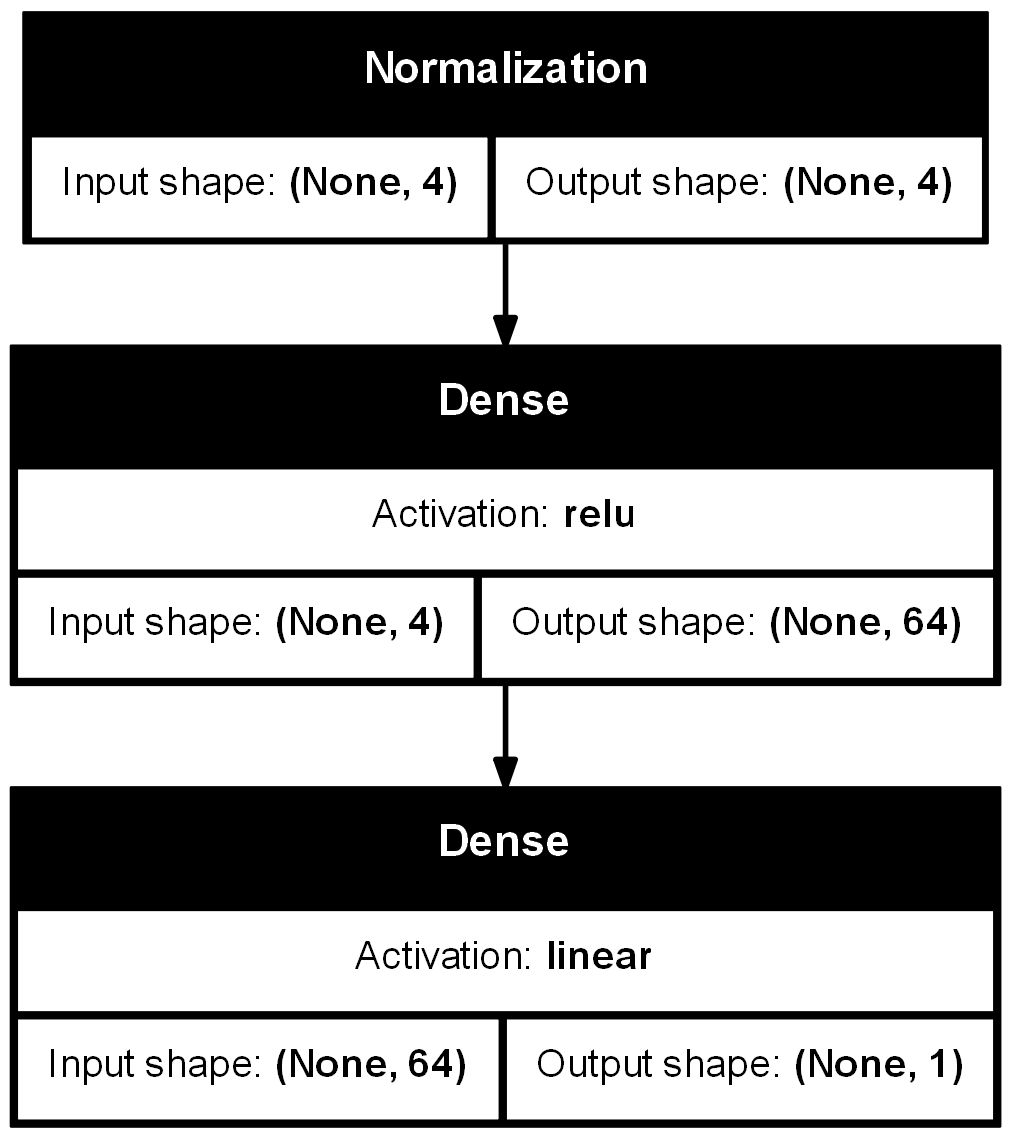
\includegraphics[width=\linewidth]{images/Results/Neural Net/1HL/structure.png}
      \caption{Δομή Νευρωνικού δικτύου με $1$ κρυφό στρώμα}
      \label{fig:Neural Network Structure with 1 Hidden layer}
  \end{minipage}
  \hfill
  \begin{minipage}{0.4\textwidth}
      \centering
      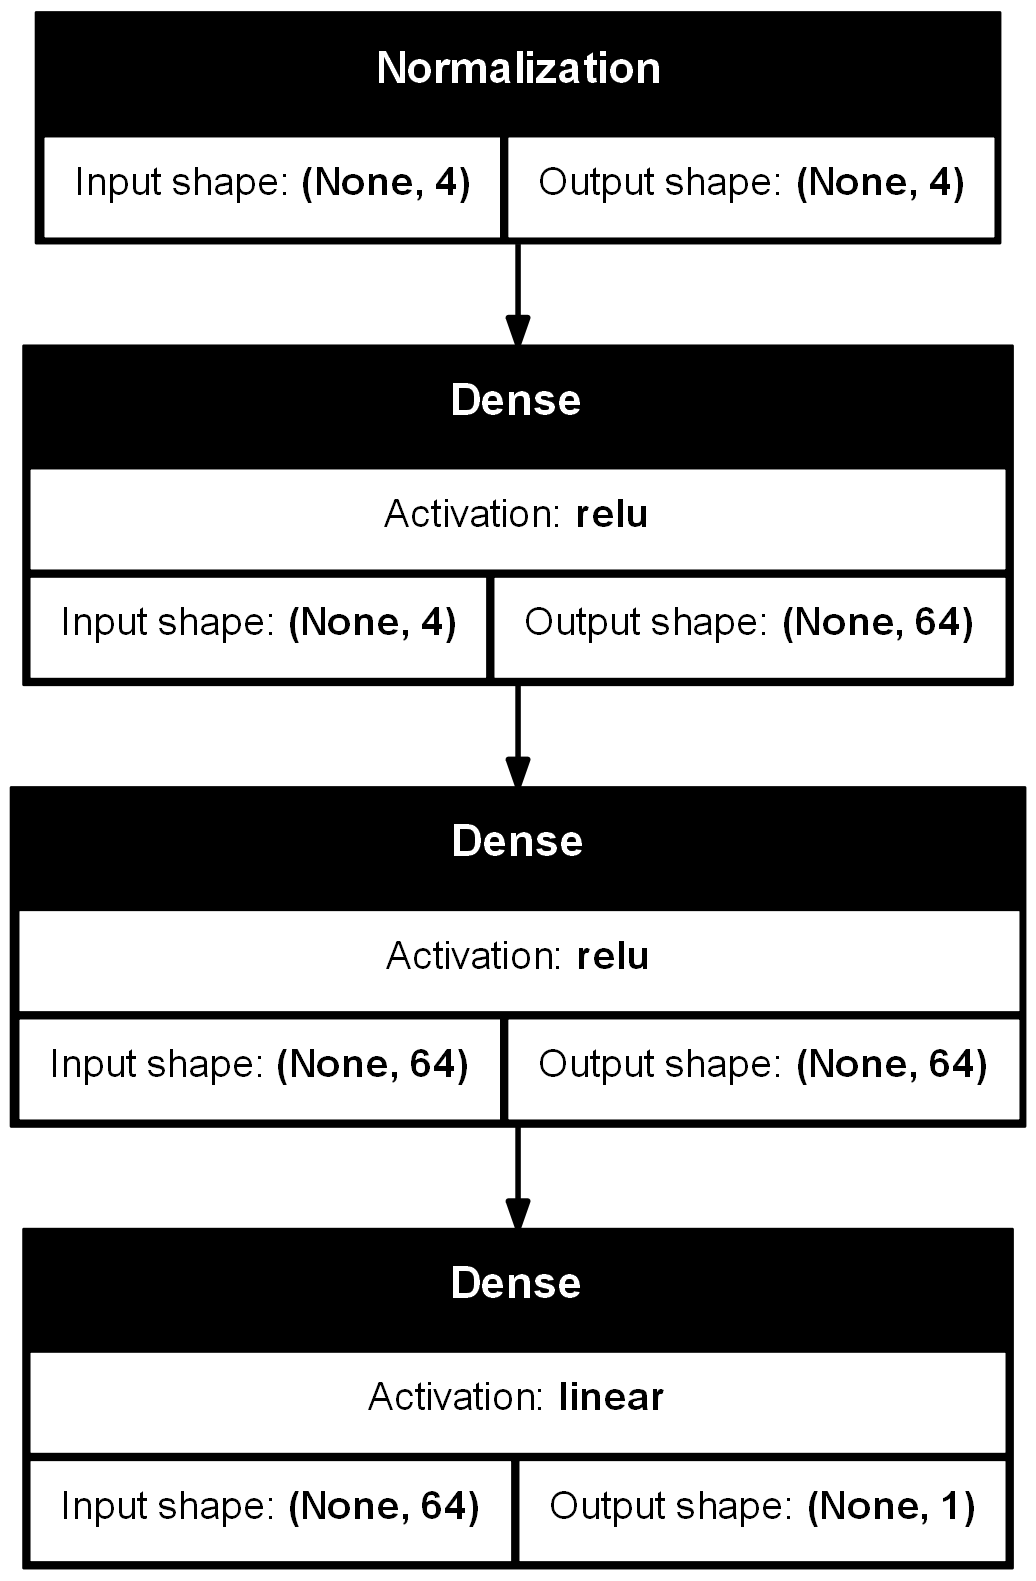
\includegraphics[width=\linewidth]{images/Results/Neural Net/2HL/structure.png}
      \caption{Δομή Νευρωνικού δικτύου με $2$ κρυφά στρώματα}
      \label{fig:Neural Network Structure with 2 Hidden layer}


  \end{minipage}
\end{figure}

\begin{figure}[H]
  \centering
  \begin{minipage}{0.4\textwidth}
      \centering
      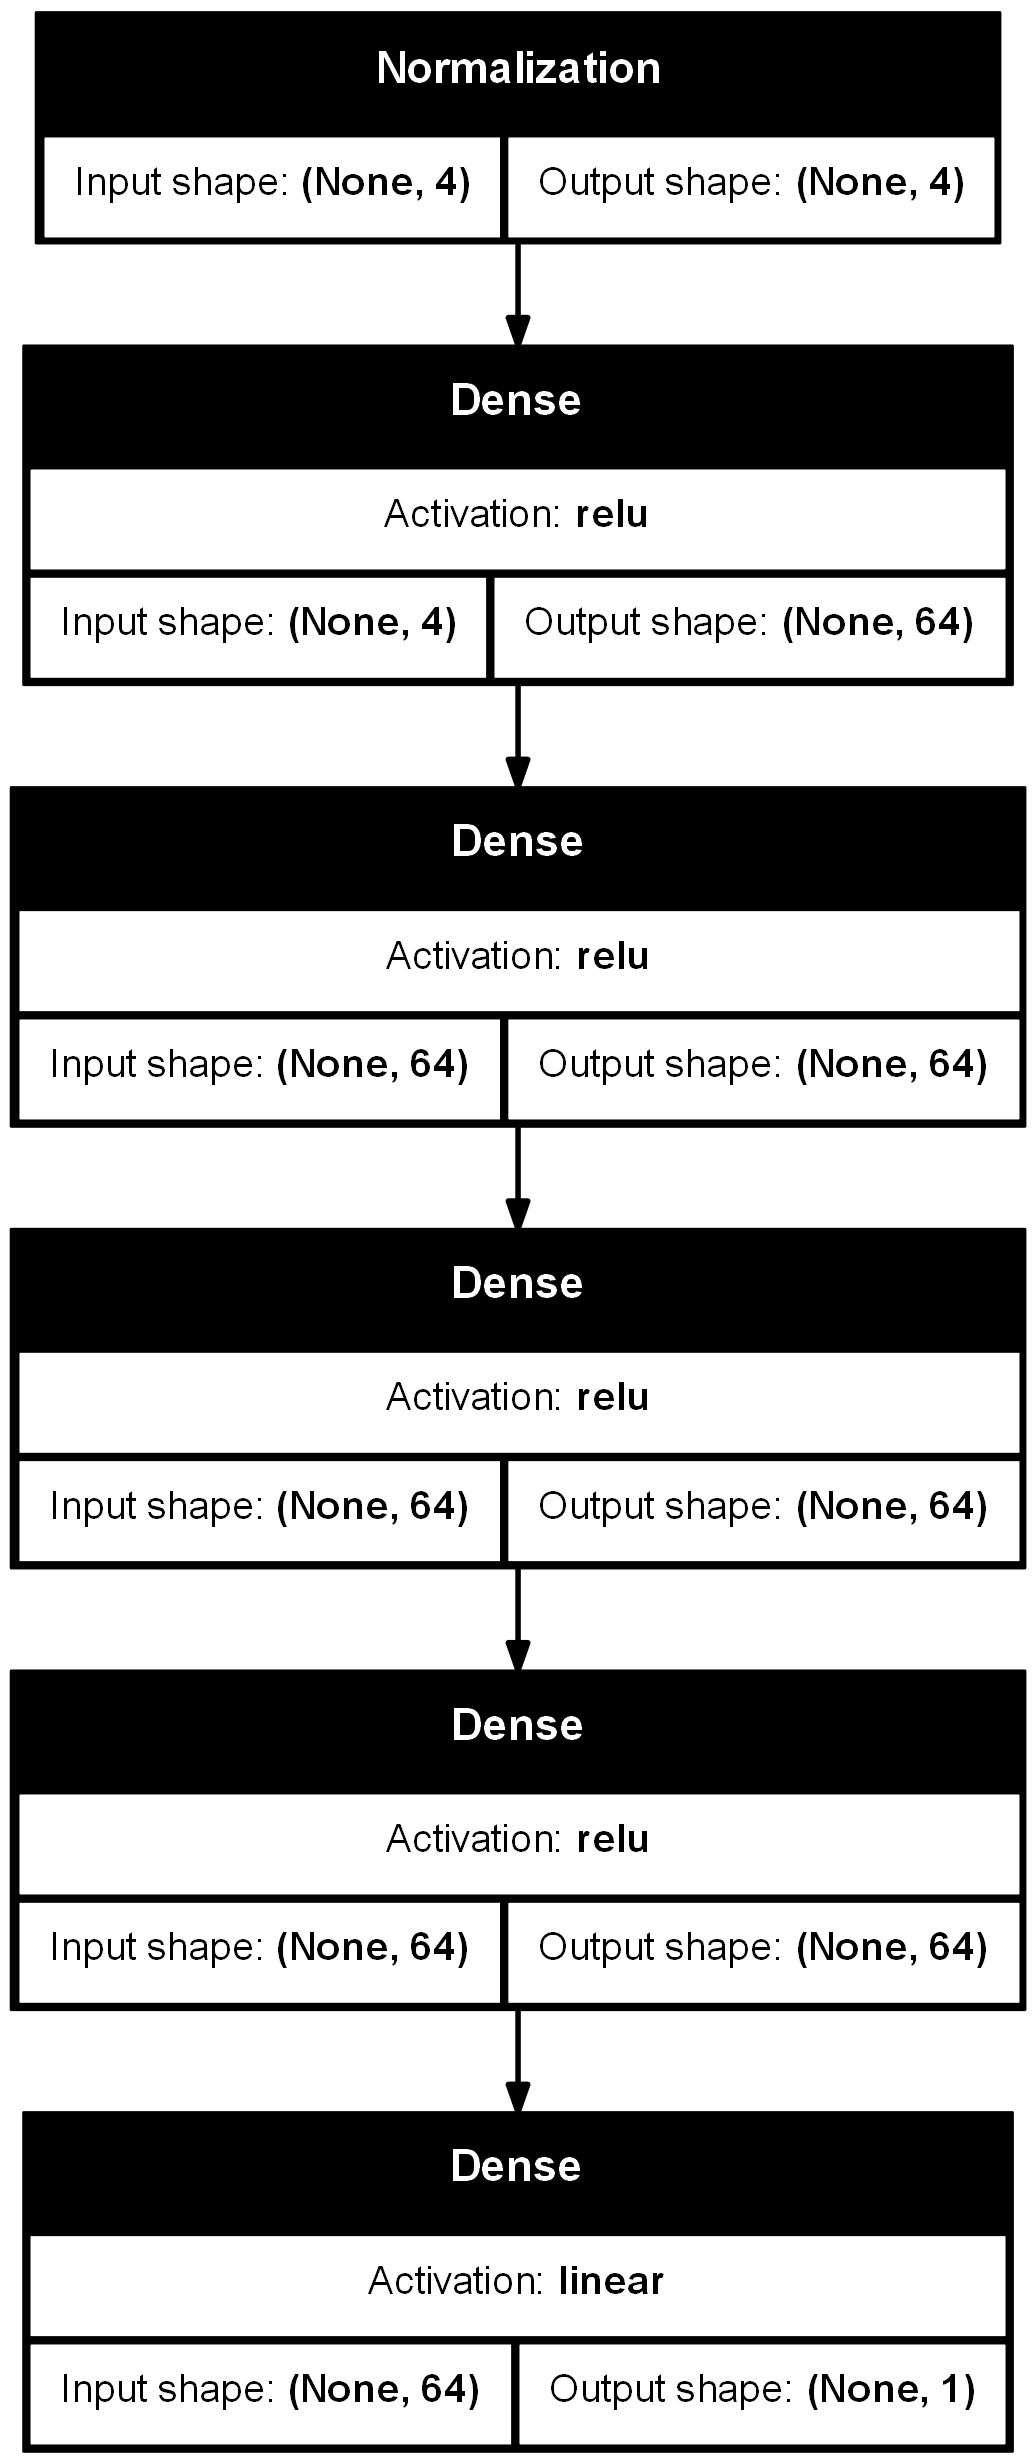
\includegraphics[width=\linewidth]{images/Results/Neural Net/4HL/structure.png}
      \caption{Δομή Νευρωνικού δικτύου με $4$ κρυφά στρώματα}
      \label{fig:Neural Network Structure with 4 Hidden layer}
  
    \end{minipage}
  \hfill
  \begin{minipage}{0.4\textwidth}
      \centering
      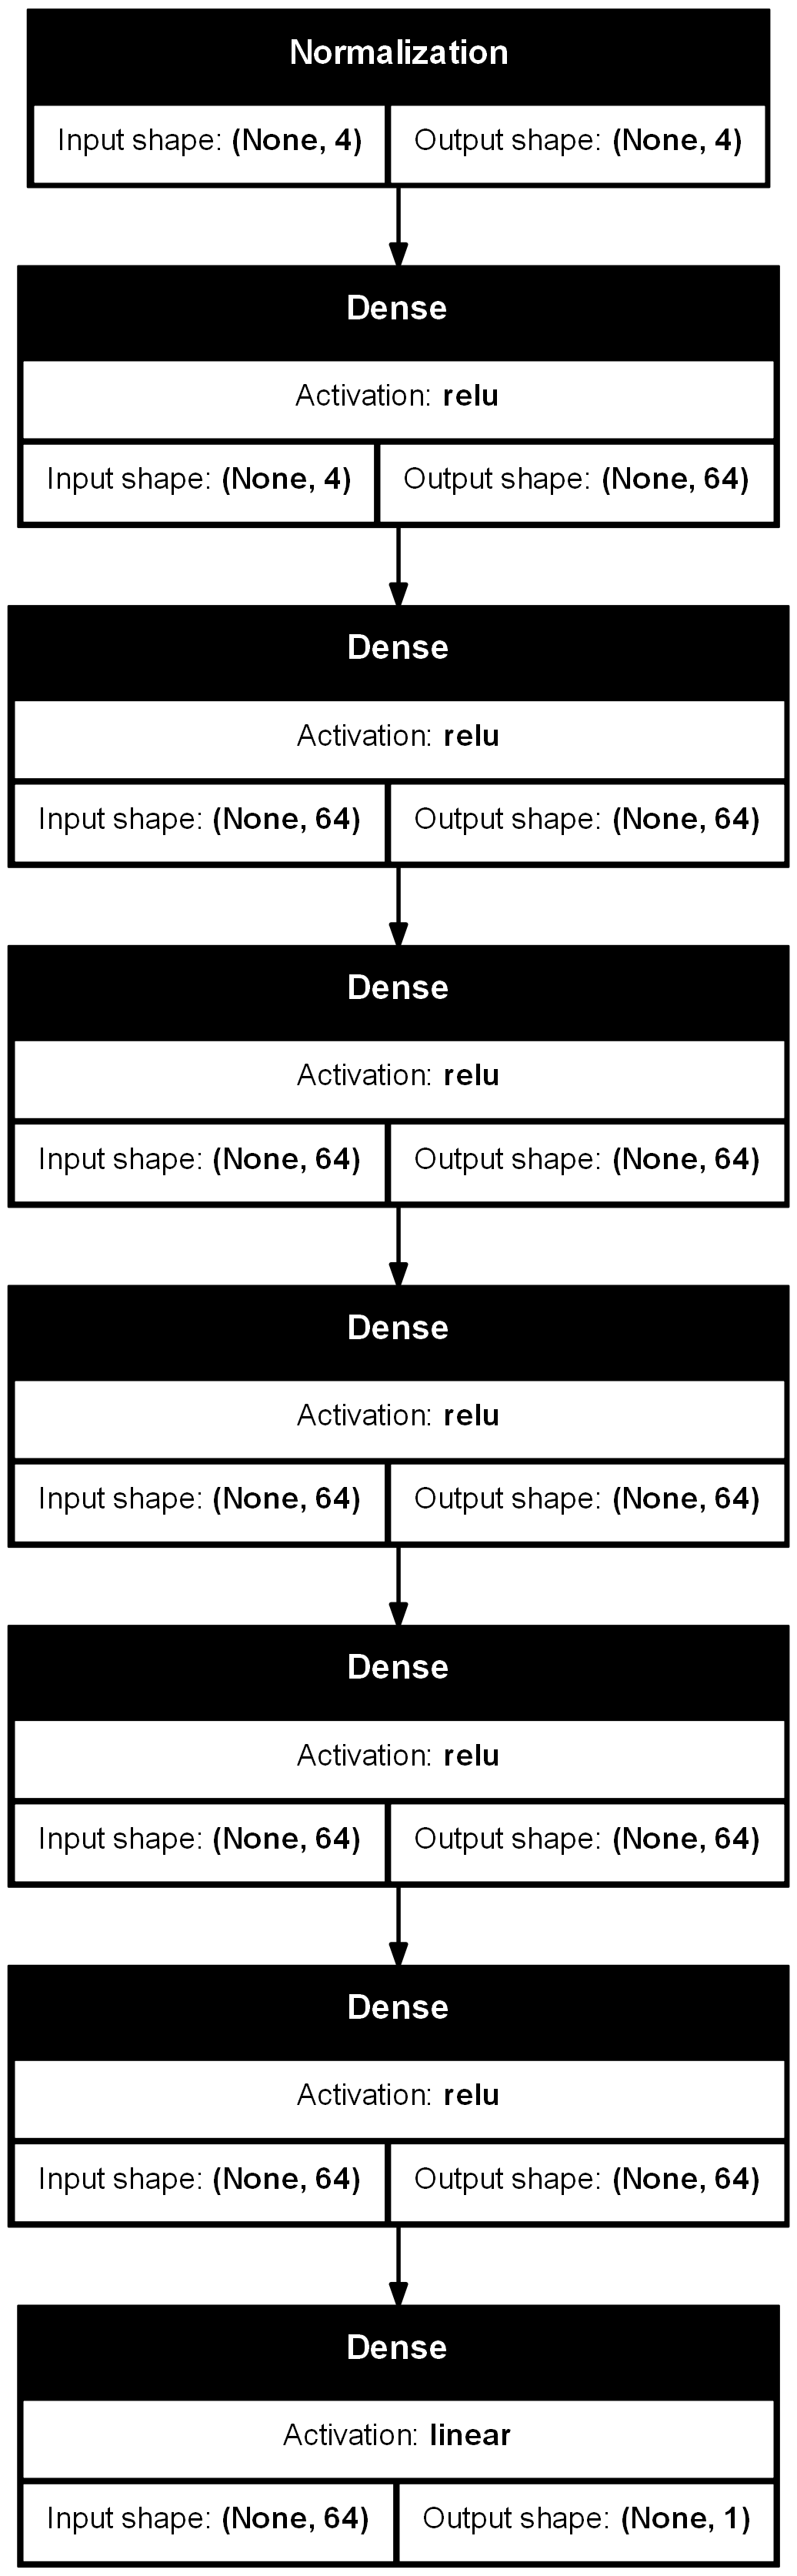
\includegraphics[width=\linewidth]{images/Results/Neural Net/6HL/structure.png}
      \caption{Δομή Νευρωνικού δικτύου με $6$ κρυφά στρώματα}
      \label{fig:Neural Network Structure with 6 Hidden layer}

  \end{minipage}
\end{figure}


\subsubsection{Συνάρτηση Απώλειας (\textlatin{Loss Function})}

Η συνάρτηση απώλειας που επιλέχθηκε για αυτήν την εφαρμογή είναι το \textlatin{Mean Average Error}, που περιγράφεται στην Εξίσωση \eqref{eq:MAE}, καθώς είναι εύκολη στην ερμηνεία της, έχει τις ίδιες μονάδες με τη μεταβλητή εξόδου και είναι ανθεκτική σε \textlatin{outlier} δεδομένα.

\subsubsection{\textlatin{Optimizer}}

Ο βελτιστοποιητής που επιλέχθηκε είναι ο \textlatin{Adam}, ο οποίος είναι ευρέως χρησιμοποιούμενος και θεωρείται ένας από τους καλύτερους βελτιστοποιητές, με ρυθμό εκμάθησης 0.01.

\subsubsection{\textlatin{hyperparameter Tuning}}
\label{Hyper-Parameter-Tuning}

Τέλος, κατασκευάζεται ένα μοντέλο του οποίου η δομή καθορίζεται από τον αλγόριθμο \textlatin{HyperBand}. Το μοντέλο είναι ελεύθερο να επιλέξει τις ακόλουθες υπερ-παραμέτρους:

\begin{itemize}
\item
  Τον αριθμό των Κρυφών Στρωμάτων μεταξύ 1 και 10.
\item
  Τον αριθμό των Νευρώνων για κάθε στρώμα από ένα διακριτό σύνολο τιμών
  \[\left\{ 2^{i} \right\}, \ \text{με}\ i = 1,2,\ldots ,10\]
\item
  Τη συνάρτηση ενεργοποίησης κάθε στρώματος:  \textlatin{ReLu, tanh,} ή \textlatin{Leaky ReLu}.
\item
  Τον  ρυθμό εκμάθησης του βελτιστοποιητή.
\end{itemize}

Η δομή αυτού του μοντέλου δεν είναι γνωστή σε αυτή τη φάση, καθώς είναι προϊόν της διαδικασίας βελτιστοποίησης. Γι' αυτό το λόγο θα παρουσιαστεί στην ενότητα αποτελεσμάτων.

Τα αποτελέσματα των Νευρωνικών Δικτύων παρουσιάζονται στην \autoref{neural-network-prediction-results}
